\documentclass[12pt,a4paper]{report}

    \newcommand{\varTitle}{Geotechnical Simulations with Moose}
    \newcommand{\varAuthor}{Jörg Meier}
    \newcommand{\varDate}{27.01.2025}

    % General document formatting
    \usepackage[margin=0.7in]{geometry}
    \usepackage[parfill]{parskip}
    \usepackage[utf8]{inputenc}
    \usepackage[]{mdframed}
    \usepackage{tikz}
    \usetikzlibrary{shapes.geometric, arrows, arrows.meta, chains, positioning}
    \usepackage{graphicx}
    \usepackage[edges]{forest}
    \usetikzlibrary{decorations.pathreplacing}

    % tables
    \usepackage{tabularx,array,booktabs,multirow}
    \newcolumntype{Y}{>{\centering\arraybackslash}X} % for centering tables in tabularx
    \usepackage{makecell}

    % Related to math
    \usepackage{amsmath,amssymb,amsfonts,amsthm}

    % make links clickable
    \usepackage{hyperref}
    \hypersetup{
        colorlinks    = true,    % Colours links instead of ugly boxes
        urlcolor      = blue,    % Colour for external hyperlinks
        linkcolor     = black,   % Colour of internal links
        bookmarksopen = true,
        citecolor     = black     % Colour of citations
    }
    \usepackage[nameinlink,noabbrev]{cleveref}

    \newcommand*{\shortautoref}[1]{%
        \begingroup
        \def\sectionautorefname{sec.}%
        \def\subsectionautorefname{sec.}%
        \autoref{#1}%
        \endgroup
    }

    \newcommand{\light}[1]{\textcolor{gray}{#1}}

    % Other packages
    \usepackage[inline]{enumitem}
    \usepackage{soul}   %for highlighting text
    % \usepackage{layouts}
    \usepackage{fontawesome5}

    % captions
    \usepackage{caption}
    \captionsetup{justification=raggedright,singlelinecheck=false}
    \usepackage{subcaption}

    % colors
    \usepackage{xcolor}
    \definecolor{dkgreen}{rgb}{0,0.6,0}
    \definecolor{gray}{rgb}{0.5,0.5,0.5}
    \definecolor{mauve}{rgb}{0.58,0,0.82}

    % code listings
    \usepackage{listings}
    \usepackage{textcomp} % for for straight single quotes (upquote=true)
    \lstdefinelanguage{Moose}{
        sensitive=f,%
        morecomment=[l]{\#},% comments
        morekeywords={true,false},%
        morestring=[b]{"},% strings with double quote
        morestring=[b]{'},% strings with single quote
        upquote=true, % for straight single quotes (see https://tex.stackexchange.com/questions/145416/how-to-have-straight-single-quotes-in-lstlistings)
        morecomment=[s][\color{blue}\ttfamily]{\[}{\]},% block names and block endings
        morecomment=[s][\color{BlueViolet}\ttfamily]{\$\{}{\}},% references to variables etc. ${...}
        literate= %{=}{{\color{blue}= }}1
                 {á}{{\'a}}1 {é}{{\'e}}1 {í}{{\'i}}1 {ó}{{\'o}}1 {ú}{{\'u}}1
                 {Á}{{\'A}}1 {É}{{\'E}}1 {Í}{{\'I}}1 {Ó}{{\'O}}1 {Ú}{{\'U}}1
                 {à}{{\`a}}1 {è}{{\`e}}1 {ì}{{\`i}}1 {ò}{{\`o}}1 {ù}{{\`u}}1
                 {À}{{\`A}}1 {È}{{\`E}}1 {Ì}{{\`I}}1 {Ò}{{\`O}}1 {Ù}{{\`U}}1
                 {ä}{{\"a}}1 {ë}{{\"e}}1 {ï}{{\"i}}1 {ö}{{\"o}}1 {ü}{{\"u}}1
                 {Ä}{{\"A}}1 {Ë}{{\"E}}1 {Ï}{{\"I}}1 {Ö}{{\"O}}1 {Ü}{{\"U}}1
                 {â}{{\^a}}1 {ê}{{\^e}}1 {î}{{\^i}}1 {ô}{{\^o}}1 {û}{{\^u}}1
                 {Â}{{\^A}}1 {Ê}{{\^E}}1 {Î}{{\^I}}1 {Ô}{{\^O}}1 {Û}{{\^U}}1
                 {ã}{{\~a}}1 {ẽ}{{\~e}}1 {ĩ}{{\~i}}1 {õ}{{\~o}}1 {ũ}{{\~u}}1
                 {Ã}{{\~A}}1 {Ẽ}{{\~E}}1 {Ĩ}{{\~I}}1 {Õ}{{\~O}}1 {Ũ}{{\~U}}1
                 {œ}{{\oe}}1 {Œ}{{\OE}}1 {æ}{{\ae}}1 {Æ}{{\AE}}1 {ß}{{\ss}}1
                 {ű}{{\H{u}}}1 {Ű}{{\H{U}}}1 {ő}{{\H{o}}}1 {Ő}{{\H{O}}}1
                 {ç}{{\c c}}1 {Ç}{{\c C}}1 {ø}{{\o}}1 {Ø}{{\O}}1 {å}{{\r a}}1 {Å}{{\r A}}1
                 {€}{{\euro}}1 {£}{{\pounds}}1 {«}{{\guillemotleft}}1
                 {»}{{\guillemotright}}1 {ñ}{{\~n}}1 {Ñ}{{\~N}}1 {¿}{{?`}}1 {¡}{{!`}}1 ,%
        alsoletter={=!},%
        morekeywords=[2]{=,!include},%
        keywordstyle=[2]{\color{blue}},%
        %https://tex.stackexchange.com/questions/217505/listings-color-numbers-only-out-of-keywords
    }[keywords,comments,strings]

    \lstset{frame=tb,
        language=Moose,
        aboveskip=3mm,
        belowskip=3mm,
        showstringspaces=false,
        columns=flexible,
        basicstyle={\small\ttfamily},
        numbers=none,
        numberstyle=\tiny\color{gray},
        keywordstyle=\color{blue},
        commentstyle=\color{dkgreen},
        stringstyle=\color{mauve},
        breaklines=true,
        breakatwhitespace=true,
        tabsize=3,
        % deletekeywords={from,in,and},
        % morekeywords={function,Algorithm,algorithm, then,do},
    }

    % awesomebox
    \usepackage{awesomebox}

    % todo
    \setlength {\marginparwidth }{2cm}
    \usepackage{xargs}                      % Use more than one optional parameter in a new commands
    \usepackage[dvipsnames]{xcolor}  % Coloured text etc.
    \usepackage[colorinlistoftodos,prependcaption,textsize=tiny]{todonotes}
    \newcommandx{\unsure}[2][1=]{\todo[linecolor=red,backgroundcolor=red!25,bordercolor=red,#1]{#2}}
    \newcommandx{\change}[2][1=]{\todo[linecolor=blue,backgroundcolor=blue!25,bordercolor=blue,#1]{#2}}
    \newcommandx{\info}[2][1=]{\todo[linecolor=OliveGreen,backgroundcolor=OliveGreen!25,bordercolor=OliveGreen,#1]{#2}}
    \newcommandx{\improvement}[2][1=]{\todo[linecolor=Plum,backgroundcolor=Plum!25,bordercolor=Plum,#1]{#2}}
    \newcommandx{\thiswillnotshow}[2][1=]{\todo[disable,#1]{#2}}
    \newcommandx{\todoinline}[2][1=]{
        {\hbadness=10000 \hfuzz=\maxdimen{\todo[inline,linecolor=Plum,backgroundcolor=Plum!25,bordercolor=Plum,#1]{#2}}}
        % \errmessage{#2}
        % \GenericError{9}{#2}{0}{1}
        % \GenericInfo{9}{#2}
        % \PackageWarning{ToDo}{#2}
        % \typeout{Package ToDo Warning: #2}\typeout{}
        % \typeout{Package ToDo Info: #2}\typeout{}
    }

    \NewDocumentCommand{\codeword}{v}{%
        \texttt{\textcolor{blue}{#1}}%
    }

    % Bulleted command: insert a sing bulleted item without any margins
    \newcommandx{\bulleted}[1]{%
        \begin{minipage}[t]{\linewidth}
            \begin{itemize}[nosep, leftmargin=1em, labelwidth=*,align=left]
                \item #1
            \end{itemize}
        \end{minipage}
    }

    \usepackage{filemod}

    \tikzstyle{startstop} = [rectangle, rounded corners, minimum width=3cm,
    minimum height=1cm, text centered, draw=black]
    \tikzstyle{process} = [rectangle, minimum width=3cm,
    minimum height=1cm, text centered, draw=black]
    \tikzstyle{decision} = [diamond, minimum width=3cm,
    minimum height=1cm, text centered, draw=black]
    \tikzstyle{arrow} = [thick, ->, >=stealth]

    % physial units
    \usepackage{siunitx}
    \DeclareSIUnit\year{a}
    \DeclareSIUnit\metreabovesealevel{\text{m ü.M.}}
    \DeclareSIUnit\ton{\text{t}}
    \DeclareSIUnit\DOF{\text{DOF}}

    % attach files
    \usepackage{currfile}
    \usepackage{attachfile}

    \newcommandx{\fileattachment}[2]{\textattachfile[color=0 0 0]{#1}{\faFile*[regular] #2}}

    % comments
    % \usepackage[opacity=0]{pdfcomment}
    % {\pdftooltip[style = mathpopup]{ \mu_\mathrm{f} }{ dynamic viscosity of the fluid }}

\title{\varTitle}

\author{\varAuthor}

\date{\varDate}

% References
\usepackage[square,sort,comma,numbers,sectionbib]{natbib}
\usepackage{multibib}
\newcites{Publications}{Publications}
% \newcites{Standards}{Standards and Recommendations}

\begin{document}

% awesomebox: override default box with to avoid overfull \hbox warning
\setlength{\aweboxcontentwidth}{0.81\linewidth}

\lstset{language=[Sharp]C,,basicstyle=\footnotesize\ttfamily,showspaces=false,showtabs=false,,breaklines=true,showstringspaces=false,breakatwhitespace=true, escapeinside={(*@}{@*)}}

%\maketitle
\begin{titlepage}
    \begin{flushright}
        
\includegraphics[width=4.5cm]{img/gruner.pdf}
    \end{flushright}
    \begin{center}
        \vspace*{5cm}

        {\Huge\textbf{\varTitle}}

        \vspace{5cm}
        %Upgrade Report

        \large{-- DRAFT --}

        \vfill

        \large{This whitepaper collects information and code \\
            for geotechnical simulations with the software Moose.}

        \vfill

        \textbf{\varAuthor}

        \vspace{0.8cm}

        Gruner AG, Geotechnical Engineering\\
        Basel, Switzerland\\

        \vspace{1cm}
        \href{https://github.com/jmeier/geotechnical-simulations-with-moose}{github.com/jmeier/geotechnical-simulations-with-moose}\\
        \varDate\\

        \vspace{1cm}
        License: CC-BY-SA-4.0

    \end{center}
\end{titlepage}

\tableofcontents

\chapter{Introduction}
\label{chap:introduction}
The open-source, parallel finite element framework Moose
(\url{mooseframework.inl.gov}) can also be used to perform geotechnical
simulations. This document aims to collect options and techniques that are
suitable for creating such geotechnical simulations with mosses. Main focus are
quasi-static simulations.

This document is primarily intended as a collection of information rather than
a textbook or step-by-step guide. As such, it is intended to be a 'living'
document that will be continually edited and updated.


\chapter{General Remarks}
\label{chap:general}
\section{Sign convention}
\label{chap:sign-convention}

% https://github.com/idaholab/moose/discussions/20999
% https://github.com/idaholab/moose/discussions/29182#discussioncomment-11456527

In the [SolidMechanics] module and the [PorousFlow] module the sign convention
is as follows:

\begin{itemize}
      \item Positive strain is extensional, which (usually) results from a positive
            (tensile) stress.
      \item Negative strain is compressional, which (usually) results from a negative
            (compressive) stress.
      \item Compressive pore-pressures (e.g. below a free water table) have a positive
            sign.
      \item Suction is represented by pore-pressures having a negative sign.
\end{itemize}


\chapter{Model Configuration}
\label{chap:setup}
\section{Strain calculation}
\label{chap:model-configuration-strain}

In the
\href{https://mooseframework.inl.gov/modules/solid_mechanics/}{'solid\_mechanics'}
module, Moose supports three different types of
\href{https://mooseframework.inl.gov/modules/solid_mechanics/Strains.html}{strain}
calculation:
\begin{itemize}
  \item {Small Linearized Total Strain}
  \item {Incremental Small Strains}
  \item {Finite Large Strains}
\end{itemize}

\begin{lstlisting}[language=perl, caption={Setting up incremental small strains within the Physics/SolidMechanics block},label={setup-incremental-small-strains}]
[Physics]
  [SolidMechanics]
    [QuasiStatic]
      [./all]
        strain = SMALL
        incremental = true
        (*@{\raisebox{-1pt}[0pt][0pt]{$\vdots$}}@*)
      []
    []
  []
[]
\end{lstlisting}

\section{Stress calculation}
\label{chap:model-configuration-stress}

\href{https://mooseframework.inl.gov/modules/solid_mechanics/Stresses.html}{Stresses.html}

The stress calculation chosen by the user must be compatible with the strain
calculation (\autoref{chap:model-configuration-strain}).

ComputeFiniteStrainElasticStress for incremental and finite strain
formulations.

\section{Fixation of the model boundaries}
\label{chap:model-configuration-boundary-fixities}

Fix the model boundaries (usually all boundaries are only fixed in the
direction of the normal and the lower boundary can also be fixed horizontally).

(to be written)

\chapter{Geometry}
\label{chap:geometry}
\section{General considerations on geometry}
\label{geometry-general}

When modelling geotechnical problems, it is often desirable to make a
meaningful geometric abstraction to avoid time-consuming modelling, but also to
avoid inaccuracies due to oversimplification. However, experience shows that
the effort involved in creating such a model geometry should not be
underestimated and that the models consist of a large number of individual
parts and components - often called ‘geometrical objects’. Some of these
objects have trivial shapes (e.g. rectangular surfaces for a sheet pile wall
segment), others can have non-trivial curvilinear boundaries (e.g. geological
bodies). All of these objects must be shaped to fit each other (without gaps or
overlaps) and together form the FE model. Usually, geotechnical models are
managed (e.g materials, staging, etc) on the level of these objects.

\section{‘Subdomains’ resp. ‘Blocks’}
\label{geometry-blocks-and-subdomains}

In Moose, so-called ‘subdomains’ are one of the central elements for the setup
and management of models. For example, materials are not assigned directly to
the FE elements, but to one or several ‘subdomains’. The same applies to
kernels, variables and many other Moose objects. The FE elements are also
assigned to subdomains, whereby each FE element can only be associated with one
subdomain. The entirety of the Moose objects and settings assigned to a
subdomain thus defines the element type and mechanical behaviour of all FE
elements within this subdomain. Therefore, a Moose model consists of at least
one ‘subdomain’. Conversely, it is necessary to create at least one subdomain
for each element type and physical material.

It is worth mentioning that FE elements that are assigned to a subdomain can,
but do not have to, be geometrically connected. The bodies built up by the FE
elements of a subdomain may therefore also have openings or internal cavities
or form several individual bodies. With this concept, a subdomain must be
understood as a logical, rather than a geometric, organisational entity.

Due to the use of \href{https://libmesh.github.io/}{libmesh} by Moose, the term
‘block’ is used as a synonym for ‘subdomain’ in many places.

To simplify the handling of construction stages, it has also proved useful to
further subdivide element sets into individual subdomains so they match the
‘geometrical objects’ mentioned before so they can to be used independently
during the simulation (e.g. deactivated or activated at different times). This
document follows this approach that Moose models are managed on the basis of
subdomains/blocks.

As the shape of these individual parts and components directly influences the
shape of the FE elements they are build of, further prerequisites must be
considered during geometrisation: For instance, as few ‘unfavourably shaped’
(e.g. too acute-angled) FE elements as possible should result in order to avoid
numerical instabilities or load increments that are too small. A common reason
for acute-angled elements and large numbers of elements are corner or end
points that are close together and unfavourable intersections of the objects.
Another requirement for geometrisation is that the number of FE elements should
remain within a range that enables acceptable calculation times.

\section{Getting the mesh into Moose}
\label{geometry-getting-the-mesh-into-moose}

Although Moose's ‘Mesh System’ provides a variety of tools for generating FE
meshes on the basis of input file commands, the creation of geometrically
complex models with these commands is often confusing and error-prone.
% https://mooseframework.inl.gov/syntax/Mesh/index.html

Therefore, the mesh including all subdomains and FE-elements is prepared
outside of Moose and imported using the \codeword{FileMeshGenerator}. The
\href{https://gmsh.info/doc/texinfo/gmsh.html#MSH-file-format}{MSH file format}
has proven itself in this context. One possible workflow is to create the
geometry of the subdomains in \href{https://blender.org}{Blender}, then
generate the mesh using \href{https://gmsh.info/}{gmsdh} and save it as an MSH
file. See listing \autoref{geometry-FileMeshGenerator} for the code required in
a Moose input file for the import of an MSH file.
% \href{https://mooseframework.inl.gov/source/meshgenerators/FileMeshGenerator.html}{FileMeshGenerator}

\begin{lstlisting}[language=Moose, float, caption={Read mesh from a file},label={geometry-FileMeshGenerator}]
[Mesh]
    [file]
        type = FileMeshGenerator
        file = "source.msh"
    []
    second_order = true
[]
\end{lstlisting}

\section{Lower dimensional blocks in MSH files}
\label{geometry-MSH}

A notable quirk of the MSH file format when used with Moose is the definition
of lower dimensional blocks. The term ‘lower dimensional blocks’ is used here
to describe subdomains with FE elements with a lower dimensionality (e.g.
shells and beams in a model with 3D solid elements). The MSH file format makes
no internal distinction as to whether blocks with lower dimensional elements
are to be interpreted as a side-set or as a ‘real’ element block. To introduce
this distinction, Moose recognises the codeword
\codeword{lower_dimensional_block} (although this codeword is not an official
part of the MSH file format). If this codeword is found in the line of an entry
in the \codeword{$PhysicalNames}, Moose assumes that this block does not
represent a sideset, but contains lower dimensional elements. As shown in
\autoref{geometry-MSH-LowerDimBlock} the codeword may be just appended at the
end of the line (without beeing part of the name of the physical name) or even
be part of the physical name itself.

\begin{lstlisting}[float, caption={Fragment of an MSH file containing ‘lower dimensional blocks’},label={geometry-MSH-LowerDimBlock}]
$MeshFormat
4.1 0 8
$EndMeshFormat
$PhysicalNames
(*@{\raisebox{-1pt}[0pt][0pt]{$\vdots$}}@*)
0 1 "PointA"                                         (*@{$\leftarrow$ side-set (node)}@*)
1 2 "topleftedge"                                    (*@{$\leftarrow$ side-set (line)}@*)
1 3 "lineSignPole000" lower_dimensional_block        (*@{$\leftarrow$ block with beam-elements}@*)
1 4 "lineSignPole001_lower_dimensional_block"        (*@{$\leftarrow$ block with beam-elements}@*)
2 5 "BoundaryZMin"                                   (*@{$\leftarrow$ side-set (surface)}@*)
2 6 "Sign" lower_dimensional_block                   (*@{$\leftarrow$ block with shell-elements}@*)
(*@{\raisebox{-1pt}[0pt][0pt]{$\vdots$}}@*)
\end{lstlisting}

\section{Choice of element types}
\label{geometry-element-types}

For obvious reasons, the element types of the individual subdomains must be
compatible with each other (e.g. the number and distribution of nodes must
match, etc). Given the often complex geometry of geotechnical models (see
\autoref{geometry-general}), elements with triangular faces are often
preferred. In this case, volume elements are correspondingly tetrahedral (TET)
and surface elements are triangular (TRI). However, since linear TET and TRI
elements (TET4 and TRI3) have very poor numerical properties (e.g.
unrealistically high stiffness, locking), ‘quadratic’ elements (TET10 and TRI6)
must be used. This leads to the commonly used compatible element types for
tetrahedral/triangular discretisation show in
\autoref{tab:geometry-TET-TRI-elements}.

\begin{table}
    \begin{tabularx}{\textwidth}{@{}lXl@{}}
        \hline
        Subdomain type
                             &
        Element type
                             &
        Comments
        \\

        \hline
        volume
                             &
        TET10
                             &
        tetrahedral element with 10 nodes and 4 integration points
        \\

        surface (e.g. shell) & TRI6  & triangular element with 6 nodes \\

        line (e.g. beam)     & EDGE3 & line element with 3 nodes       \\

        \hline
    \end{tabularx}
    \caption{Commonly used compatible element types for tetrahedral/triangular discretisation}
    \label{tab:geometry-TET-TRI-elements}
\end{table}

Currently, Moose has full support for TET10 elements, but not for EDGE3 and
TET6 elements. EDGE3 and TRI6 elements can currently be used in a Moose-app by
cloning the following Moose code-plugins as a ‘contrib’:

\begin{description}[font=$\bullet$~\normalfont]
    \item [beams:] \href{https://github.com/Kavan-Khaledi/moose-codeplugin-beam}{github.com/Kavan-Khaledi/moose-codeplugin-beam}
    \item [shells:] \href{https://github.com/Kavan-Khaledi/moose-codeplugin-shell}{github.com/Kavan-Khaledi/moose-codeplugin-shell}
\end{description}

\section{Groups of geometrical objects}
\label{geometry-groups}

Moose does not explicitly support groups geometrical objects but allows to
create variables in the input file holding names of several objects on one hand
and to use these variables directly for block-restriction (e.g. assignment of
materials).

Due to the fact that Moose throws an error if unused variables are found in the
input file, but the user may want to define groups even if they are not
(currently) used, it has proven useful to add 'fake users' using a
ParsedFunction as shown in \autoref{geometry-moose-variable-groups}.

\begin{lstlisting}[language=Moose, float, caption={Moose input file fragment: variable holding several block names and fake-user},label={geometry-moose-variable-groups}]
[Mesh]
    # Variable holding names of all blocks with volumes
    Volumes = 'Base Column Suzanne'
[]

[Functions]
    # Fake user for the variable above
    [FakeUser_Volumes]
        type = ParsedFunction
        expression = 'a'
        symbol_names = 'a'
        symbol_values = '1'
        control_tags = ${Mesh/Volumes}
    []
[]
\end{lstlisting}


\chapter{Modelling of geometric entities, structures, loads, etc.}
\label{chap:entities}
\section{Overview}
\label{chap:entities-overview}

This chapter collects information on how different types of geometric entities,
structures, loads etc. can be modelled. \autoref{tab:entities-overview}
contains a list of common geotechnical components and associated options that
can be used for modelling them.

\begin{table}
    \begin{tabularx}{\textwidth}{@{}lXl@{}}
        \hline
        Entity
         &
        Options for Modelling
         &
        Reference
        \\

        \hline
        soil volume
         &
        \bulleted{cluster of volume elements}
         &
        \shortautoref{chap:entities-volume}
        \\

        \hline
        excavation pit wall
         &
        \bulleted{shell elements}
         &
        \shortautoref{chap:entities-shell}
        \\

         &
        \bulleted{cluster of volume elements in case of a 'thick' wall (e.g. slurry wall, bored pile wall)}
         &
        \shortautoref{chap:entities-volume}
        \\

        \hline
        concrete volume

         &
        \bulleted{cluster of volume elements}
         &
        \shortautoref{chap:entities-volume}
        \\

         &
        \bulleted{shell elements in case of a 'thin' walls}
         &
        \shortautoref{chap:entities-shell}
        \\

        \hline
        sprayed concrete
         &
        \bulleted{shell elements}
         &
        \shortautoref{chap:entities-shell}
        \\

        \hline
        pile, soil nail
         &
        \bulleted{cluster of volume elements in case of a pile with large diameter (e.g. bored pile)}
         &
        \shortautoref{chap:entities-volume}
        \\

        %  &
        % \bulleted{embedded beams}
        %  &
        % \shortautoref{chap:entities-embedded-beams}
        % \\

        \hline
        prop
         &
        \bulleted{spring between nodes}
         &
        \shortautoref{chap:entities-springs}
        \\

         &
        \bulleted{fixed end spring}
         &
        \shortautoref{chap:entities-fixed-end-springs}
        \\

         &
        \bulleted{beam}
         &
        \shortautoref{chap:entities-beams}
        \\

        \hline
        ground anchor
         &
        \bulleted{spring between nodes + (embedded) beam}
         &
        \shortautoref{chap:entities-springs}
        \\

        \hline
    \end{tabularx}
    \caption{Selected geotechnical entities and their respective modelling}
    \label{tab:entities-overview}
\end{table}

\section{Entities}
% \label{chap:entities}

\subsection{Volumes}
\label{chap:entities-volume}

To model a volume, such as a soil volume, concrete volume, etc., the following
is required:

\begin{description}[font=$\bullet$~\normalfont]
    \item [subdomain:] A subdomain of FE-elements of an appropriate element type (e.g. TET10).
    \item [materials:] Assignment of Moose materials defining the constitutive behaviour.
\end{description}

\subsection{FixedEndSprings}
\label{chap:entities-fixed-end-springs}

Fixed end springs are currently not directly supported by Moose. As a
workaround one can define a spring between nodes
(\autoref{chap:entities-springs}) and fix the other node.

\href{https://mooseframework.inl.gov/source/nodalkernels/CoupledForceNodalKernel.html}{CoupledForceNodalKernel}

\href{https://onlinelibrary.wiley.com/doi/pdf/10.1002/pamm.202200045}{pamm.202200045}

\subsection{Springs between nodes (NodeToNodeAnchors)}
\label{chap:entities-springs}

% Springs between nodes are directly supported by Moose. 
(to be written)

mastodon:
\href{https://mooseframework.inl.gov/mastodon/source/materials/LinearSpring.html}{LinearSpring}

\subsection{Beams (line element)}
\label{chap:entities-beams}

To model beams, the following is required:

\begin{description}[font=$\bullet$~\normalfont]
    \item [subdomain:] A subdomain of FE-elements of an appropriate element type (e.g. EDGE3).
    \item [materials:] Assignment of Moose materials defining the constitutive behaviour of the beam.
\end{description}

Currently, Moose has no support for appropriate beam elements and materials for
EDGE3. In your MooseApp, the beam material for EDGE may be included as an
‘contrib’ by cloning into
\href{https://github.com/Kavan-Khaledi/moose-codeplugin-beam}{github.com/Kavan-Khaledi/moose-codeplugin-beam}

% \subsection{EmbeddedBeams (line element)}
% \label{chap:entities-embedded-beams}

\subsection{Shell (surface element)}
\label{chap:entities-shell}

To model shells (or "plates"), the following is required:

\begin{description}[font=$\bullet$~\normalfont]
    \item [subdomain:] A subdomain of FE-elements of an appropriate element type (e.g. TRI6).
    \item [materials:] Assignment of Moose materials defining the constitutive behaviour of the shell.
\end{description}

Currently, Moose has no support for appropriate shell elements and materials
for TRI6. In your MooseApp, the shell material for TRI6 may be included as an
‘contrib’ by cloning into
\href{https://github.com/Kavan-Khaledi/moose-codeplugin-shell}{github.com/Kavan-Khaledi/moose-codeplugin-shell}

\subsection{Interfaces (surface element)}

(to be written)

\subsection{Contact}

(to be written)

\subsection{Pore Pressure Boundaries}

(to be written)

\chapter{Initial Conditions}
\label{chap:initial}
\section{Initial conditions for Moose objects}
\label{chap:IC-moose-objects}

For definition of the initial (starting) conditions for the variables a Moose
simulation the \href{https://mooseframework.inl.gov/syntax/ICs}{ICs system} is
to be used.

(to be written)

\section{Gravitation and initial stress state}
\label{chap:IC-stress-state}

The initial stress state of geotechnical simulations is often non-trivial. This
is because the section of geosphere to be modelled often has a history of
millions of years under different loading conditions, including gravity and
tectonical processes. In addition, the Earth's surface is often non-horizontal,
so that stress trajectories near the surface are oriented accordingly.
Furthermore, the initial stress state may be anisotropic with a specific
orientation. Gravity and the initial stress state are normally taken into
account by means of:

\begin{itemize}
    \item Definition of appropriate displacement boundary conditions for the model (see
          \autoref{chap:model-configuration-boundary-fixities}).
    \item Activation of gravitational body force (see
          \autoref{chap:IC-stress-state-gravity}).
    \item Definition of eigenstrains from the inital stress field (e.g. using
          \href{https://mooseframework.inl.gov/source/materials/ComputeEigenstrainFromInitialStress.html}{ComputeEigenstrainFromInitialStress},
          see \autoref{chap:IC-stress-state-simple} and
          \autoref{chap:IC-stress-state-anisotropic}).
\end{itemize}

\subsection{Gravity}
\label{chap:IC-stress-state-gravity}

To consider gravity, the following aspects must be included in the model:
\begin{itemize}
    \item When compiling the MooseApp: As the effect of gravity is taken into account in
          interaction with the material density, the Moose module \codeword{MISC} must be
          active in addition to the Moose module \codeword{SOLID_MECHANICS}.
    \item Gravity must be activated in the input file. This is done by adding a special
          kernel of the type \codeword{Gravity} as shown in
          \autoref{initial-conditions-gravity}. The direction and strength of the
          gravitational field is to be defined here.
    \item The materials must be assigned a material density
          (\autoref{initial-conditions-density}).
\end{itemize}

\begin{lstlisting}[language=perl, float, caption={Gravity kernel in a Moose inut file},label={initial-conditions-gravity}]
[Kernels]
    [gravity]
        type = Gravity
        use_displaced_mesh = false
        variable = disp_z
        value = -9.81
    []
[]
\end{lstlisting}

\begin{lstlisting}[language=perl, float, caption={Assignment of a density to subdomain ‘block1’},label={initial-conditions-density}]
[Materials]
    [undrained_density]
      type = GenericConstantMaterial
      block = 'Block1'
      prop_names = density
      prop_values = 0.0025
    []
[]
\end{lstlisting}

{\hfuzz=20pt
\subsection{Initial stress state using ComputeEigenstrainFromInitialStress}
}
\label{chap:IC-stress-state-simple}

This initial stress state corresponds to the ‘geostatic stress state’ in the
uninfluenced homogeneous half-space (or a section thereof) under the effect of
gravity, which can be represented analytically in a stress point as follows:

\begin{equation}
    \sigma_{ini,vert}=\sigma_{ini,vert,h=0}+\gamma h
\end{equation}
\begin{equation}
    \sigma_{ini,horiz}=\sigma_{ini,vert} K_0 \quad \text{with } \quad K_0 = 1-\sin\varphi
\end{equation}

In these equations, $\gamma=\rho g$ corresponds to the weight of the soil, $h$
to the overburden height, $\sigma_{ini,vert,h=0}$ to the vertical stress at
$h=0$ and $K_0$ to the earth pressure coefficient. This earth pressure
coefficient is usually estimated as a function of the angle of internal
friction $\varphi$ (simplified equation according to Jaky).

\autoref{initial-conditions-ComputeEigenstrainFromInitialStress} shows the
definition of a geostatic initial stress state using two functions
\codeword{ini_xx_yy} and \codeword{ini_zz} and their subsequent use in a
\codeword{ComputeEigenstrainFromInitialStress}.

\begin{lstlisting}[language=perl, float, caption={Definition of a geostatic initial stress state using ‘ComputeEigenstrainFromInitialStress’ },label={initial-conditions-ComputeEigenstrainFromInitialStress}]
[Functions]
    [ini_xx_yy]
      type = ParsedFunction
      vars = 'sig_top   z_top   rho      g    k0 '
      vals = '-1.5      0       0.0025   10   0.3'
      value = '(sig_top - rho * g * (z_top - z)) * k0'
    []
    [ini_zz]
      type = ParsedFunction
      vars = 'sig_top   z_top   rho      g'
      vals = '-1.5      0       0.0025   10'
      value = '(sig_top - rho * g * (z_top - z))'
    []
[]
  
[Materials]
    [strain]
      type = ComputeIncrementalSmallStrain
      volumetric_locking_correction=false
      eigenstrain_names = ini_stress
    []
    [ini_stress]
      type = ComputeEigenstrainFromInitialStress
      eigenstrain_name = ini_stress
      initial_stress = 'ini_xx_yy 0 0   0 ini_xx_yy 0   0 0 ini_zz'
    []
[]
\end{lstlisting}

\subsection{Initial stress state for anisotropic stresses}
\label{chap:IC-stress-state-anisotropic}

Align the model to the orientation of the initial stresses

(to be written)

\subsection{Checking the initial stress state}
\label{chap:IC-check}

In geotechnics, the initial state including the initial stress state should be
in equilibrium. Therefore, in a first time step without any changes to the
model ‘nothing’ should happen (only neglectable deformations and changes in the
stress field).

This can be checked by introducing such a time step without any changes as a
first time step and assessing the system response (e.g. in Paraview).


\chapter{Construction Stages}
\label{chap:stages}
\section{General comments on construction stages}
\label{chap:stages-general}

The type of geotechnical simulation primarily discussed in this document aims
to model a construction process. Accordingly, such a simulation must reproduce
the various stages of construction over time. Since this document assumes that
Moose models are organised on the basis of subdomains
(\autoref{geometry-blocks-and-subdomains}), the state changes also refer
primarily to adjustments that affect entire subdomains.

The most common state changes in this context are:

\begin{itemize}
      \item Activating FE-elements (e.g. installation of sheet piles is usually modelled by
            activating the corresponding set ot FE-elements,
            \autoref{chap:stages-element-activation-deactivation})
      \item Deactivating FE-elements (e.g. excavation of a soil volume is usually modelled
            by deactivating the corresponding set of FE-elements,
            \autoref{chap:stages-element-activation-deactivation})
      \item Replacing FE-elements (e.g. installation of a slurry wall modelled via volume
            elements leads to the need to replace the soil volume with the volume
            representing the slurry wall, \autoref{chap:stages-element-replacement})
      \item Adjusting external loads (e.g. loads are used to model various influences. As
            these influences change over time, the corresponding loads have to be adjusted,
            \autoref{chap:stages-loads})
      \item Adjusting prestress (e.g. for props and stand anchors the prestress is to be
            adjusted, \autoref{chap:stages-prestress})
\end{itemize}

As a consequence of the Moose input file concept, these status adjustments must
be triggered at various points in an input file if Moose is used ‘out of the
box’. To provide a more centralised way of defining construction stages, the
\codeword{[Stages]} MooseApp code plugin linked below can be used:

\href{https://github.com/jmeier/moose-codeplugin-stages}{github.com/jmeier/moose-codeplugin-stages}

This document primarily describes the procedure for the definition of
construction stages, with the use of the \codeword{[Stages]} code plugin where
applicable. The procedure without this plugin is only mentioned in selected
places.

\section{Apprupt vs. gradual changes}
\label{chap:stages-gradual-changes}

For transient simulations, the speed at which changes are applied in the model
usually matter.

(to be written)

\section{Activating and deactivating FE-elements}
\label{chap:stages-element-activation-deactivation}

As mentioned in \autoref{geometry-blocks-and-subdomains}, Moose models are
organized and managed by means of subdomains. By assigning FE elements and
materials to a subdomain, for example, the behaviour of these FE elements is
defined. However, Moose does not offer the option of activating or deactivating
FE elements or subdomains during a simulation run. However, Moose allows FE
elements to be reassigned from one subdomain to another during a simulation run
using the
\href{https://mooseframework.inl.gov/syntax/MeshModifiers/index.html}{MeshModifiers}
system.

On the other hand, Moose allows for subdomains to exist without kernels,
variables, materials and other Moose objects, but for FE elements to be present
in these subdomains. FE-elements in those subdomains ‘without physics’ will
simply be ignored my Moose.

Activation and deactivation of FE elements can thus be modelled by combining
the option to have subdomains ‘without physics’ and the option to reassign FE
elements to another subdomain. For deactivation FE elements are moved from a
subdomain ‘with physics’ to a subdomain ‘without physics’. For activation vice
versa.

ToDo:
\begin{itemize}
      \item Activation / Deactivation with [Stages]
      \item Ramp up / ramp down material properties, \autoref{chap:stages-gradual-changes}
\end{itemize}

\section{Replacing FE-elements}
\label{chap:stages-element-replacement}

(to be written)

\section{Adjusting external loads}
\label{chap:stages-loads}

(to be written)

\section{Adjusting prestress}
\label{chap:stages-prestress}

(to be written)

\chapter{Material Models for Soil and Rock}
\label{chap:materials}
\section{Preliminary remarks on the material models}
\label{chap:material-remarks}

The built-in library of material models suitable for modelling soil and rock is
currently very limited.

\section{NEML2}
\label{chap:material-NEML2}

Moose supports the use of materials defined by means of the external material
modeling library \href{https://github.com/reverendbedford/neml2}{NEML2}
(Messner and Hu). Details on the integration of NEML2 into Moose are not scope
of this document and can be found in the corresponding
\href{https://mooseframework.inl.gov/moose/modules/solid_mechanics/NEML2.html}{corresponding
    section of the Moose documentation}.

\section{Mohr-Coulomb (linear-elastic ideal-plastic)}
\label{chap:material-mohr-coulomb}

(to be written)


\chapter{Proven Patterns}
\label{chap:patterns}
\section{Partial input files}
\label{chap:patterns-partial-input-files}

When a Moose model is defined as an
\href{https://mooseframework.inl.gov/application_usage/input_syntax.html}{‘input
    file’} (usually with the file extension ‘*.i’), the size of such an input file
can quickly grow to several hundred lines, even without the model geometry.
Editing and troubleshooting becomes correspondingly confusing. Moose therefore
also supports ‘partial input files’, where other input files can be called up
from a ‘central’ input file. For example, the material parameters or variables
with groups of geometrical objects could be maintained in a separate file.

The recommented option is to use the \codeword{!include} keyword within the
input file. This option is shown in \autoref{patterns-include}. Please note,
that the neither path not filename are allowed to contain a newline character,
\codeword{#} character, or \codeword{[} character.

\begin{lstlisting}[language=perl, caption={Include anpther input file},label={patterns-include}]
!include "path/to/file.i"
\end{lstlisting}

The alternative and not recommented option is to call a Moose app with several
input files as arguments. These input files are interpreted by simply
concatenating them. This functionality was included in Moose for test purposes,
but is not suitable for productive models, as this call may not be not
documented and may not be reproducible:

\codeword{./moose-opt -i input1.i -i input2.i -i input3.i}

\section{Physical units}
\label{chap:patterns-physical-units}

In Moose, all numerical values must be entered in a system of units which is
consistent in itself - but which is selected by the user. Without additional
options, the user must enter a number in the input file without a unit being
explicitly labelled.

In addition, Moose - like other FE programmes - calculates internally with a
finite precision. To avoid rounding errors and inaccuracies in the numerical
calculation, it is therefore important that the numerical values entered are
not too large. With a careful choice of the system of physical units, the user
can avoid such numerical problems.

From the user's point of view, the challenge is to enter the numerical values
in the ‘correct’ system of physical units everywhere in the input file. This
conversion and the non-trivial verifiability is a source of error that should
not be underestimated, particularly in the case of physical units with a time
reference. Experience shows, that this is a frequent source of problems!

To mitigate this source of error, Moose offers the
‘\href{https://mooseframework.inl.gov/source/utils/Units.html}{MooseUnits}’
unitily. In the input file this utility allows to convert the unit ‘on the
fly’. The input file fragment shown in
\autoref{patterns-physical-units-example1} converts \SI{1000e3}{\kN\per\m^2}
into \SI{}{\MN\per\m^2} and assigns the result to the variable \codeword{E}.

\begin{lstlisting}[language=perl, caption={Converting \SI{1000e3}{\kN\per\m^2} into
    \SI{}{\MN\per\m^2}},label={patterns-physical-units-example1}]
E = ${units 1000E3 kN/m^2 -> MN/m^2}
\end{lstlisting}

In connection with variables holding the desired physical units for the model
this utility can be used to enforce a consistent system of physical units in
the input file and the user can simultaneously use the physical units of his
source data (for better verifiability).
\autoref{patterns-physical-units-example2} shows the use of a variable used to
hold the desired model unit for lengths.

\begin{lstlisting}[language=perl, caption={Using a variable to hold the physical unit for lengths},label={patterns-physical-units-example2}]
# variable holding the pyhsical unit for lengths
modelunit_length = 'm'

# conversion of 10 mm into the desired model unit (m)
a = ${units 10 mm -> ${modelunit_length}}
\end{lstlisting}

A full set of pysical units can be setup as shown in
\autoref{patterns-physical-unit-set}. If not all variables are used in the
input file, Moose will issue an error. This can be avoided by adding fake-users
to the variables.

\begin{lstlisting}[language=perl, caption={Set of consistent physical units in a Moose inut file},label={patterns-physical-unit-set}]
# model units
modelunit_length = 'm'
modelunit_time = 's'    #s = seconds, h = hours, day = days
modelunit_mass = 'kg' # Mg = tons; Gg = kilotons

# derived units (this may be moved into a !include)
modelunit_force  = ${raw ${modelunit_mass} * ${modelunit_length} / ${modelunit_time} ^ 2}
modelunit_pressure = ${raw ${modelunit_force} / ${modelunit_length} ^ 2}
modelunit_acceleration = ${raw ${modelunit_length} / ${modelunit_time} ^ 2}
modelunit_density = ${raw ${modelunit_mass} / ${modelunit_length} ^ 3}

# Fake userss for the variables above
[Functions]
    [FakeUser_modelunit_force]
        type = ParsedFunction
        expression = 'a'
        symbol_names = 'a'
        symbol_values = '1'
        control_tags = ${modelunit_force}
    []
    (*@{\raisebox{-1pt}[0pt][0pt]{$\vdots$}}@*)
[]
\end{lstlisting}

A selection of model unit combinations can be found in
\autoref{tab:model-units}.

\begin{table}[htbp]
    \centering
    \caption{selection of model unit combinations and derived units}
    \label{tab:model-units}
    \begin{tabularx}{\textwidth}{
            >{\hsize=0.10\hsize\linewidth=\hsize}Y
            >{\hsize=0.10\hsize\linewidth=\hsize}Y
            >{\hsize=0.10\hsize\linewidth=\hsize}Y
            |
            >{\hsize=0.20\hsize\linewidth=\hsize}Y
            >{\hsize=0.20\hsize\linewidth=\hsize}Y
            >{\hsize=0.15\hsize\linewidth=\hsize}Y
            >{\hsize=0.15\hsize\linewidth=\hsize}Y}
        \hline
        Length                                                                             &
        Time                                                                               &
        Mass                                                                               &
        Force                                                                              &
        Pressure                                                                           &
        Acceleration                                                                       &
        Density                                                                              \\

        \hline

        \si[per-mode = symbol]{\metre}                                                     &
        \si[per-mode = symbol]{\second}                                                    &
        \si[per-mode = symbol]{\kilogram}                                                  &
        \si[per-mode = symbol]{\kilogram\cdot\metre\per\second\squared} = \si{\newton}     &
        \si[per-mode = symbol]{\newton\per\metre\squared} \light{= \si{\pascal}}           &
        \si[per-mode = symbol]{\metre\per\second\squared}                                  &
        \si[per-mode = symbol]{\kilogram\per\metre\cubed}                                    \\

        \si[per-mode = symbol]{\metre}                                                     &
        \si[per-mode = symbol]{\second}                                                    &
        \si[per-mode = symbol]{\ton}                                                       &
        \si[per-mode = symbol]{\ton\cdot\metre\per\second\squared} = \si{\kilo\newton}     &
        \si[per-mode = symbol]{\kilo\newton\per\metre\squared} \light{= \si{\kilo\pascal}} &
        \si[per-mode = symbol]{\metre\per\second\squared}                                  &
        \si[per-mode = symbol]{\ton\per\metre\cubed}                                         \\

        \hline
    \end{tabularx}
\end{table}

\section{Moose code plugins}
\label{chap:patterns-code-plugins}

If MooseApps are extended with new MooseObjects that should be shared with
other users, e.g. in workgroups, the need arises to be able to transfer this
functionality to other MooseApps as a plug-in. Preferably without having to
manually copy and adapt many code files. Furthermore, it is often good if there
is independent source code management or versioning. The idea is to realise
such code plugins for MooseApps as git submodules.

To address this need and provide versioning via a git submodule, Moose code
plugins to be found in the following link can be used:
\href{https://github.com/jmeier/mooseapp-code-plugin}{github.com/jmeier/mooseapp-code-plugin}

\chapter{Postprocessing}
\label{chap:postprocessing}
\section{\todomarker Paraview}
\label{chap:postprocessing-paraview}

Directly use the ExodusII-files produced by Moose.

(to be written)

\section{\todomarker Blender using the BVtkNodes addon}
\label{chap:postprocessing-blender}

The \href{https://github.com/tkeskita/BVtkNodes}{BVtkNodes addon} for Blender
that wraps the Visualization Toolkit (VTK) library for scientific visualization
in Blender.

(to be written)

\section{Directly accessing ExodusII files}
\label{chap:postprocessing-ExodusII}

The primary output format of Moose is ExodusII. Accessing the data directly in
this format is therefore a logical step. To work with ExodusII-files under
Windows, one might want to compile the corresponding code in the
\href{https://github.com/sandialabs/seacas}{seacas-repo} under Windows. The
step by step instructions on how to compile ExodusII for windows can be found
here: \href{https://github.com/sandialabs/seacas/discussions/375}{seacas\#375}.


\chapter{Outlook}
\label{chap:outlook}
The following topics are currently not covered, but may be of interest:

\begin{itemize}
    \item Restart a simulation run from a given time step.
    \item Branching simulations runs (closely related to restarting simulation runs)
    \item Changing the solver and convergence criteria depending on (simulation) time
\end{itemize}

\chapter{References}
\label{chap:references}

\nocitePublications{*}
\bibliographystylePublications{plainnat}
\bibliographyPublications{src/references/publications.bib}

% \nociteStandards{*}
% \bibliographystyleStandards{plainnat}
% \bibliographyStandards{src/references/standards.bib}

\appendix
\chapter{Fully Saturated Undrained Compression}
\label{app:fully-saturated-undrained-compression}
\section{Problem statement}

A one-dimensional compression test of a $\SI{6}{\metre} \times \SI{6}{\metre}
    \times \SI{6}{\metre}$ fully saturated block is to be simulated as a variant of
an Oedometer test. While the (vertical) sides are fixed horizontally and the
bottom is fixed vertically, the top surface is lowered by
$\SI{0.01}{\metre}=\SI{1}{\centi\metre}$. Initially, the block is loaded only
by gravity. The soil material is assumed to be purely linear elastic and fully
saturated with water. Material parameters are given in
\autoref{fully-saturated-undrained-compression:material-parameters}. Stiffness
of the material had been chosen in accordance with Opalinus clay (a sedimentary
rock), while permeability should been chosen high enough to avoid significant
time-dependent effects.

The effective vertical stress $\sigma'_{zz}$ and pore pressure $u$ are to be
determined as simulation result at the top of the block.

\begin{table}[htbp]
    \centering
    \caption{Material parameters}
    \label{fully-saturated-undrained-compression:material-parameters}
    \begin{tabularx}{\textwidth}{XYY}

        \hline

        Property                               & Physical unit                                     & Value       \\

        \hline

        soil: Youngs modulus $E$               & \si[per-mode =
        symbol]{\giga\newton\per\square\metre} & \SI{18}{}                                                       \\

        soil: Poisson's ratio $\nu$            & -                                                 & \SI{0.25}{} \\

        soil: density $\rho_s$                 & \si[per-mode = symbol]{\kilogram\per\cubic\metre} &
        \SI{2500}{}                                                                                              \\

        soil: permeability $k$                 & \si[per-mode = symbol]{\square\metre}             & (realistic
        high)                                                                                                    \\

        water: bulk modulus $K_w$              & \si[per-mode =
        symbol]{\giga\newton\per\square\metre} & \SI{2.2}{}                                                      \\

        water: dynamic viscosity $\mu_w$       & \si[per-mode =
        symbol]{\milli\pascal\cdot\second}     & \SI{0.9}{}                                                      \\

        water: density $\rho_w$                & \si[per-mode = symbol]{\kilogram\per\cubic\metre} &
        \SI{998.21}{}                                                                                            \\

        porosity $n$                           & -                                                 & \SI{0.11}{} \\

        \hline
    \end{tabularx}
\end{table}

\section{Analytical solution}

For the one-dimensional deformation conditions and the linear-elastic material
behaviour defined for this problem the definition of the stiffness modulus in
\autoref{fully-saturated-undrained-compression:stiffness-modulus} holds:

\begin{equation}
    \label{fully-saturated-undrained-compression:stiffness-modulus}
    E_s = \frac{\sigma'_{zz}}{\varepsilon_{zz}} = E \cdot \frac{1 - \nu}{(1 + \nu)(1 - 2 \nu)}
\end{equation}

\begin{samepage}
    with:
    \begin{description}
        \item[$E_s$] Stiffness modulus
        \item[$\sigma'_{zz}$] effective vertical stress
        \item[$\varepsilon_{zz}$] vertical strain
        \item[$E$] Young's modulus
        \item[$\nu$] Poisson's ratio
    \end{description}
\end{samepage}

Using the values of
\autoref{fully-saturated-undrained-compression:material-parameters} for the
second part of
\autoref{fully-saturated-undrained-compression:stiffness-modulus} leads to:
\begin{equation}
    \label{fully-saturated-undrained-compression:stiffness-modulus-value}
    \begin{split}
        E_s & = E \cdot \frac{1 - \nu}{(1 + \nu)(1 - 2 \nu)}                                                                       \\
            & = \SI{18}{\si[per-mode = symbol]{\giga\newton\per\square\metre}} \cdot \frac{1 - 0.25}{(1 + 0.25)(1 - 2 \cdot 0.25)} \\
            & = \SI{21.6}{\si[per-mode = symbol]{\giga\newton\per\square\metre}}
    \end{split}
\end{equation}

Rearranging the first part of
\autoref{fully-saturated-undrained-compression:stiffness-modulus} for
$\sigma'_{zz}$ allows to estimate the effective stresses at the top of the
block:
\begin{equation}
    \label{fully-saturated-undrained-compression:effective_vertical_stress}
    \begin{split}
        \sigma'_{zz} & = E_s \cdot \varepsilon_{zz}                                                                                                                                                                               \\
                     & = \SI{21.6}{\si[per-mode = symbol]{\giga\newton\per\square\metre}} \cdot \frac{ \SI{0.01}{\metre} \cdot \SI{6}{\metre} \cdot \SI{6}{\metre} }{ \SI{6}{\metre} \cdot  \SI{6}{\metre} \cdot  \SI{6}{\metre}} \\
                     & = \SI{0.036}{\si[per-mode = symbol]{\giga\newton\per\square\metre}} = \SI{3.6E4}{\si[per-mode = symbol]{\kilo\newton\per\square\metre}}
    \end{split}
\end{equation}

\vspace{1em}

To estimate the pore-pressure,
\autoref{fully-saturated-undrained-compression:pore-pressure-parameter} can be
used:

\begin{equation}
    \label{fully-saturated-undrained-compression:pore-pressure-parameter}
    % source: Förster, W. (1996): Mechanische Eigenschaften Lockergesteine. Teubner Verlag. Equation 7.65 on page 142
    C = \frac{\Delta u}{\Delta \sigma_{zz}} = \frac{1}{1 + n \cdot \frac{m_w}{m_v}}
\end{equation}
with:
\begin{description}
    \item[$C$] Pore pressure parameter
    \item[$\Delta u$] pore pressure
    \item[$\Delta \sigma_{zz}$] difference of total vertical stress, $\Delta \sigma_{zz} = \Delta (\sigma'_{zz} + u)$
    \item[$n$] Porosity
    \item[$m_w$] Coefficient of volume compressibility for water, $m_w = 1/K_w \equiv 1/{\SI[per-mode = symbol]{2.2}{\giga\newton\per\square\metre}}$
    \item[$m_v$] Coefficient of volume compressibility for the solid; here assumed to be linear-elastic and therefore not dependent on the stress and/or initial porosity: $m_v = 1 / E_s$
\end{description}

\vspace{1em}

leading to:

\begin{equation}
    % \label{fully-saturated-undrained-compression:???}
    C = \frac{1}{1 + n \cdot \frac{E_s}{K_w}} \approx 0.48\overline{076923}
\end{equation}

and due to the fact the initial stress state is Zero,
\autoref{fully-saturated-undrained-compression:pore-pressure-parameter} can be
rearranged to calculate the pore pressure $u$:

\begin{equation}
    % \label{fully-saturated-undrained-compression:???}
    u = \frac{C \cdot \Delta \sigma_{zz}}{1 - C} =
    3.\overline{3}\times\SI{E4}{\si[per-mode =
            symbol]{\kilo\newton\per\square\metre}}
\end{equation}

% \begin{equation}
%     \label{fully-saturated-undrained-compression:bulk modulus}
%     K = \frac{E}{3(1 - 2 \nu)}
% \end{equation}

\section{Numerical solution with Moose}

The system of physical units for the Moose model was set to metre
(\unit{\metre}), seconds (\unit{\second}), and tons (\unit{\ton}). Due to this,
the physical unit for stress and pore-pressures is \unit[per-mode =
    symbol]{\kilo\newton\per\square\metre}. Because of the physical unit of seconds
(\unit{\second}) and to keep model time to numbers with small magnitude, a high
permeability of $k = \qty{1E-7}{\square\metre}$ was chosen (comparable with a
gravel) and model time was set to \qty{10}{\second}.

The mesh used for Moose consists of \qty{5184}{} TET10 elements leading to
\qty{32980}{\DOF}.

Residuals for the fluid (water with a dynamic viscosity of $\mu_\mathrm{f}
    \approx \qty{1}{\milli\pascal\cdot\second} $) with an accepted pressure
gradient of $ \epsilon_\mathrm{f} \equiv \qty[per-mode =
        symbol]{10}{\pascal\per\metre} $ may be estimated as:
\begin{equation}
    \begin{split}
        R_\mathrm{f} & \approx V \cdot \kappa \cdot \epsilon_\mathrm{f} \cdot \rho_\mathrm{f} / { \mu_\mathrm{f} }                                                                                                                                        \\
                     & \approx (\qty{216}{\cubic\metre}) \cdot (\qty{1E-7}{\square\metre}) \cdot (\qty[per-mode = symbol]{10}{\pascal\per\metre}) \cdot (\qty[per-mode = symbol]{1000}{\kilogram\per\cubic\metre}) / (\qty{1}{\milli\pascal\cdot\second}) \\
                     & \approx \qty{2.16E+2}{\kilogram\cdot\metre\per\second}  \hspace{3.00em} \text{\light{(in SI units)}}                                                                                                                               \\
                     & \approx \qty{2.16E-1}{\ton\cdot\metre\per\second}       \hspace{3.09em} \text{\light{(in accordance with the selected model units)}}
    \end{split}
\end{equation}

% Leading to a scaling of the pore-pressure of $\sim \qty{1E+1}{}$ (calculated
% using $ 1 / R_\mathrm{f} $). In fact, for this particular model a very small
% sensitivity of the resulting pore-pressure and vertical stress on the scaling
% had been found.

For this model, variable scaling was determined as follows:
\begin{enumerate}
    \item Variable scaling of all variables (\texttt{disp\_x}, \texttt{disp\_y},
          \texttt{disp\_z}, and \texttt{porepressure}) is set to unity.
    \item\label{ite:test_run_residuals} {Using
              \texttt{Debug/show\_var\_residual\_norms = true} the residuals of the
              individual variables are printed for a test run of the model. The residuals for
              the first time step (Time Step 1) are:\vspace{0.1cm}
              \begin{mdframed}[leftmargin=0.1cm,innerleftmargin=0.1cm,topline=false,rightline=false,bottomline=false]
                  \begin{verbatim}
|residual|_2 of individual variables:
          disp_x:       19.4404
          disp_y:       19.4404
          disp_z:       110.432
          porepressure: 7.33977e-05
0 Nonlinear |R| = 1.138024e+02\end{verbatim}
              \end{mdframed}}
    \item The magnitude of the residuals in \autoref{ite:test_run_residuals} for the
          \texttt{disp}-variables are roughly the same, while the magnitude of the
          \texttt{porepressure} is much smaller. Therefore, without scaling, the
          contribution to the residual of the \texttt{porepressure} would be strongly
          underrepresented and one would need very small \texttt{abs\_norm\_tol} to make
          sure that the hydraulic equation converges. On the other hand, this may cause
          convergence problems for the displacement equations as they have larger
          residuals.\newline It is therefore advisable for this model to scale the
          \texttt{porepressure} in such a way that the associated residuals are
          comparable with those of the \texttt{disp} variables using (while leaving
          scaling of all \texttt{disp} variables at unity):
          \texttt{Variables/porepressure/scaling = 1E+5}

\end{enumerate}

In Moose, this model was calculated and analysed separately using both the
‘NEWTON’ solver and the ‘PJFNK’ solver. The Moose input files for this model
are attached to this document by the name of
‘fully-saturated-undrained-compression-NEWTON.i’ and
‘fully-saturated-undrained-compression-PJFNK.i’.

\fileattachment{\currfiledir/fully-saturated-undrained-compression-NEWTON.i}{fully-saturated-undrained-compression-NEWTON.i}

\fileattachment{\currfiledir/fully-saturated-undrained-compression-PJFNK.i}{fully-saturated-undrained-compression-PJFNK.i}

Selected results of the Moose models are summarized in
\autoref{fully-saturated-undrained-compression:moose-results} (both solvers
used lead to the same results within the specified precision). Performance data
can be found in
\autoref{fully-saturated-undrained-compression:moose-performance}.

\begin{table}[htbp]
    \centering
    \caption{Selected results of the Moose models \\(identical for solvers ‘NEWTON’ and ‘PJFNK’ for the shown precision)}
    \label{fully-saturated-undrained-compression:moose-results}

    \begin{tabularx}{0.972\hsize}{
            >{\hsize=0.6\hsize\linewidth=\hsize}X
            >{\hsize=0.4\hsize\linewidth=\hsize}X}
        {\begin{tabularx}{1\linewidth}{
                     >{\hsize=0.3\hsize\linewidth=\hsize}X
                     >{\hsize=0.3\hsize\linewidth=\hsize\hspace{-5pt}}Y
                     >{\hsize=0.3\hsize\linewidth=\hsize\hspace{-5pt}}Y}
                 \toprule
                 Model response                                                                        & \multicolumn{2}{c}{Location}                     \\
                 {}                                                                                    & $z_{max}$                    & $z_{min}$         \\
                 \midrule

                 \multicolumn{3}{l}{Initial Conditions:}                                                                                                  \\
                 \hspace{1em} $\sigma'_{zz}$ (\unit[per-mode = symbol]{\kilo\newton\per\square\metre}) & \qty{\pm0.0}{}               & \qty{-90.0}{}     \\
                 \hspace{1em} $u$            (\unit[per-mode = symbol]{\kilo\newton\per\square\metre}) & \qty{\pm0.0}{}               & \qty{-60.0}{}     \\

                 {}                                                                                    & {}                           & {}                \\

                 \multicolumn{3}{l}{Boundary at $z_{max}$ lowered by \qty{1}{cm} ($t = \qty{11}{\second}$):}                                              \\
                 \hspace{1em} $\sigma'_{zz}$ (\unit[per-mode = symbol]{\kilo\newton\per\square\metre}) & \qty{-3.600E+4}{}            & \qty{-3.608E+4}{} \\
                 \hspace{1em} $u$            (\unit[per-mode = symbol]{\kilo\newton\per\square\metre}) & \qty{-3.335E+4}{}            & \qty{-3.341E+4}{} \\
                 \bottomrule
             \end{tabularx}}
         &
        {\raisebox{0.0mm}
                {\begin{tikzpicture}[baseline=(current bounding box.center)]
                         \node[inner sep=0pt] (ch-stresses) at (0.35,0.0) {\includegraphics[width=0.925\linewidth]{\currfiledir fully-saturated-undrained-compression.i.png}};
                         \node[draw,circle,fill=white,minimum size=.95cm,inner sep=0pt] at (+3.3,+2.2) {$z_{max}$};
                         \node[draw,circle,fill=white,minimum size=.95cm,inner sep=0pt] at (+3.1,-1.6) {$z_{min}$};
                     \end{tikzpicture}}
            }
        \\
    \end{tabularx}
\end{table}

\begin{table}[htbp]
    \centering
    \caption{Performance of Moose}
    \label{fully-saturated-undrained-compression:moose-performance}
    \begin{tabularx}{\textwidth}{
            >{\hsize=0.16\hsize\linewidth=\hsize}X
            >{\hsize=0.14\hsize\linewidth=\hsize\hspace{-5pt}}Y
            >{\hsize=0.14\hsize\linewidth=\hsize\hspace{-5pt}}Y
            >{\hsize=0.14\hsize\linewidth=\hsize\hspace{-5pt}}Y
            >{\hsize=0.14\hsize\linewidth=\hsize\hspace{-5pt}}Y
            >{\hsize=0.14\hsize\linewidth=\hsize\hspace{-5pt}}Y
            >{\hsize=0.14\hsize\linewidth=\hsize\hspace{-5pt}}Y}

        \hline

        Property              & \multicolumn{3}{c}{Solver "NEWTON"}   & \multicolumn{3}{c}{Solver
        "PJFNK"}                                                                                  \\

        {}                    &
        1 CPU                 &
        3 CPU                 &
        5 CPU                 &
        1 CPU                 &
        3 CPU                 &
        5 CPU                                                                                     \\

        \hline

        wall time             & \qty[per-mode = symbol]{105}{\second} & \qty[per-mode =
        symbol]{45}{\second}  & \qty[per-mode = symbol]{32}{\second}  & \qty[per-mode =
        symbol]{169}{\second} & \qty[per-mode = symbol]{69}{\second}  & \qty[per-mode =
        symbol]{46}{\second}                                                                      \\

        %RAM                                      &
        %\qty[per-mode = symbol]{205}{\mega\byte} &
        %\qty[per-mode = symbol]{308}{\mega\byte} &
        %\qty[per-mode = symbol]{293}{\mega\byte} &
        %\qty[per-mode = symbol]{435}{\mega\byte} &
        %\qty[per-mode = symbol]{287}{\mega\byte} &
        %\qty[per-mode = symbol]{252}{\mega\byte}   \\

        \hline
    \end{tabularx}
\end{table}

% ########################################################
% ########## Dependency on variable scaling ##############
% ########################################################
%
% the following table is commented out due to the fact, I do not see any
% impact of the variable scaling (for the values tested).
%
% The effect of scaling the ‘porepressure’ variable is shown in
% \autoref{fully-saturated-undrained-compression:tab:moose-scaling}.
%
% \begin{table}[htbp]
%     \centering
%     \caption{Effect of scaling the ‘porepressure’ variable (results at $z_{max}$)}
%     \label{fully-saturated-undrained-compression:tab:moose-scaling}
%     \begin{tabularx}{\textwidth}{
%             >{\hsize=0.30\hsize\linewidth=\hsize}X
%             >{\hsize=0.15\hsize\linewidth=\hsize\hspace{-5pt}}Y
%             >{\hsize=0.15\hsize\linewidth=\hsize\hspace{-5pt}}Y
%             >{\hsize=0.05\hsize\linewidth=\hsize\hspace{-5pt}}Y
%             >{\hsize=0.15\hsize\linewidth=\hsize\hspace{-5pt}}Y
%             >{\hsize=0.15\hsize\linewidth=\hsize\hspace{-5pt}}Y
%             >{\hsize=0.05\hsize\linewidth=\hsize\hspace{-5pt}}Y}
% 
%         \hline
% 
%         Variable ‘porepressure’                                                    &
%         \multicolumn{3}{c}{Solver "NEWTON"}                                        &
%         \multicolumn{3}{c}{Solver "PJFNK"}                                           \\
% 
%         scaling                                                                    &
%         $\sigma'_{zz}$ (\unit[per-mode = symbol]{\kilo\newton\per\square\metre})   &
%         $u$            (\unit[per-mode = symbol]{\kilo\newton\per\square\metre})   &
%         rem.                                                                       &
%         $\sigma'_{zz}$ (\unit[per-mode = symbol]{\kilo\newton\per\square\metre})   &
%         $u$            (\unit[per-mode = symbol]{\kilo\newton\per\square\metre})   &
%         rem.                                                                         \\
% 
%         \hline
% 
%         \qty[print-zero-exponent=true, print-exponent-implicit-plus=true]{1E+05}{} &
%         \qty[per-mode = symbol]{-3.600E+4}{}                                       &
%         \qty[per-mode = symbol]{+3.335E+4}{}                                       &
%         {}                                                                         &
%         \qty[per-mode = symbol]{-3.600E+4}{}                                       &
%         \qty[per-mode = symbol]{+3.335E+4}{}                                       &
%         {}                                                                           \\
% 
%         \qty[print-zero-exponent=true, print-exponent-implicit-plus=true]{1E+02}{} &
%         \qty[per-mode = symbol]{-3.600E+4}{}                                       &
%         \qty[per-mode = symbol]{+3.335E+4}{}                                       &
%         {}                                                                         &
%         \qty[per-mode = symbol]{-3.600E+4}{}                                       &
%         \qty[per-mode = symbol]{+3.335E+4}{}                                       &
%         {}                                                                           \\
% 
%         \qty[print-zero-exponent=true, print-exponent-implicit-plus=true]{1E+01}{} &
%         \qty[per-mode = symbol]{-3.600E+4}{}                                       &
%         \qty[per-mode = symbol]{+3.335E+4}{}                                       &
%         {}                                                                         &
%         \qty[per-mode = symbol]{-3.600E+4}{}                                       &
%         \qty[per-mode = symbol]{+3.335E+4}{}                                       &
%         {}                                                                           \\
% 
%         \qty[print-zero-exponent=true, print-exponent-implicit-plus=true]{1E+00}{} &
%         \qty[per-mode = symbol]{-3.600E+4}{}                                       &
%         \qty[per-mode = symbol]{+3.335E+4}{}                                       &
%         {}                                                                         &
%         \qty[per-mode = symbol]{-3.600E+4}{}                                       &
%         \qty[per-mode = symbol]{+3.335E+4}{}                                       &
%         {}                                                                           \\
% 
%         \qty[print-zero-exponent=true, print-exponent-implicit-plus=true]{1E-01}{} &
%         \qty[per-mode = symbol]{-3.600E+4}{}                                       &
%         \qty[per-mode = symbol]{+3.335E+4}{}                                       &
%         {}                                                                         &
%         \qty[per-mode = symbol]{-3.600E+4}{}                                       &
%         \qty[per-mode = symbol]{+3.335E+4}{}                                       &
%         {}                                                                           \\
% 
%         \qty[print-zero-exponent=true, print-exponent-implicit-plus=true]{1E-02}{} &
%         \qty[per-mode = symbol]{-3.600E+4}{}                                       &
%         \qty[per-mode = symbol]{+3.335E+4}{}                                       &
%         {}                                                                         &
%         \qty[per-mode = symbol]{-3.600E+4}{}                                       &
%         \qty[per-mode = symbol]{+3.335E+4}{}                                       &
%         {}                                                                           \\
% 
%         \qty[print-zero-exponent=true, print-exponent-implicit-plus=true]{1E-03}{} &
%         \qty[per-mode = symbol]{-3.600E+4}{}                                       &
%         \qty[per-mode = symbol]{+3.335E+4}{}                                       &
%         {}                                                                         &
%         \qty[per-mode = symbol]{-3.600E+4}{}                                       &
%         \qty[per-mode = symbol]{+3.335E+4}{}                                       &
%         {}                                                                           \\
% 
%         \qty[print-zero-exponent=true, print-exponent-implicit-plus=true]{1E-04}{} &
%         \qty[per-mode = symbol]{-3.600E+4}{}                                       &
%         \qty[per-mode = symbol]{+3.335E+4}{}                                       &
%         {}                                                                         &
%         \qty[per-mode = symbol]{-3.600E+4}{}                                       &
%         \qty[per-mode = symbol]{+3.335E+4}{}                                       &
%         {}                                                                           \\
% 
%         \qty[print-zero-exponent=true, print-exponent-implicit-plus=true]{1E-05}{} &
%         \qty[per-mode = symbol]{-3.600E+4}{}                                       &
%         \qty[per-mode = symbol]{+3.335E+4}{}                                       &
%         {}                                                                         &
%         \qty[per-mode = symbol]{-3.600E+4}{}                                       &
%         \qty[per-mode = symbol]{+3.335E+4}{}                                       &
%         {}                                                                           \\
% 
%         \qty[print-zero-exponent=true, print-exponent-implicit-plus=true]{1E-10}{} &
%         \qty[per-mode = symbol]{-3.600E+4}{}                                       &
%         \qty[per-mode = symbol]{+3.335E+4}{}                                       &
%         {}                                                                         &
%         \qty[per-mode = symbol]{-3.600E+4}{}                                       &
%         \qty[per-mode = symbol]{+3.335E+4}{}                                       &
%         {}                                                                           \\
% 
%         \qty[print-zero-exponent=true, print-exponent-implicit-plus=true]{1E-15}{} &
%         \qty[per-mode = symbol]{-3.600E+4}{}                                       &
%         \qty[per-mode = symbol]{+3.335E+4}{}                                       &
%         {}                                                                         &
%         \qty[per-mode = symbol]{-3.600E+4}{}                                       &
%         \qty[per-mode = symbol]{+3.335E+4}{}                                       &
%         {}                                                                           \\
% 
%         \hline
%     \end{tabularx}
%     %\raggedright
%     %(a) \texttt{-nl\_rel\_tol} = \qty{1E-6}{};
%     %(b) \texttt{-nl\_rel\_tol} = \qty{1E-7}{};
%     %(c) \texttt{-nl\_rel\_tol} = \qty{1E-8}{}
% \end{table}

% ########################################################
% ################## Memory Consumption ##################
% ########################################################
%
% /usr/bin/time -v ./shale-opt -i models/porous_flow_block/porous_flow_block.i
% 
% Performance Graph:
% --------------------------------------------------------------------------------------------------------------------------------------------------------------------------
% |                                Section                               | Calls |   Self(s)  |   Avg(s)   |    %   | Mem(MB) |  Total(s)  |   Avg(s)   |    %   | Mem(MB) |
% --------------------------------------------------------------------------------------------------------------------------------------------------------------------------
% | shaleTestApp (main)                                                  |     1 |      0.007 |      0.007 |   0.00 |       4 |    167.881 |    167.881 | 100.00 |     290 |
% |   Action::SetupMeshAction::Mesh::SetupMeshAction::act::setup_mesh    |     1 |      0.000 |      0.000 |   0.00 |       0 |      0.000 |      0.000 |   0.00 |       0 |
% |   Action::SetupMeshAction::Mesh::SetupMeshAction::act::set_mesh_base |     2 |      0.000 |      0.000 |   0.00 |       0 |      0.000 |      0.000 |   0.00 |       0 |
% |   MeshGeneratorSystem::createMeshGeneratorOrder                      |     1 |      0.000 |      0.000 |   0.00 |       0 |      0.000 |      0.000 |   0.00 |       0 |
% |   FEProblem::computeUserObjects                                      |     2 |      0.000 |      0.000 |   0.00 |       0 |      0.000 |      0.000 |   0.00 |       0 |
% |   FEProblem::computeUserObjects                                      |     3 |      0.000 |      0.000 |   0.00 |       0 |      0.000 |      0.000 |   0.00 |       0 |
% |   FEProblem::outputStep                                              |    12 |      0.002 |      0.000 |   0.00 |       0 |      0.541 |      0.045 |   0.32 |      12 |
% |   Transient::PicardSolve                                             |    11 |      0.010 |      0.001 |   0.01 |       0 |    166.360 |     15.124 |  99.09 |     117 |
% |     FEProblem::computeUserObjects                                    |    88 |      0.001 |      0.000 |   0.00 |       0 |      0.001 |      0.000 |   0.00 |       0 |
% |     FEProblem::outputStep                                            |    33 |      0.002 |      0.000 |   0.00 |       0 |      0.002 |      0.000 |   0.00 |       0 |
% |     FEProblem::solve                                                 |    11 |     70.303 |      6.391 |  41.88 |      88 |    164.285 |     14.935 |  97.86 |     117 |
% |       FEProblem::computeUserObjects                                  |    84 |      0.000 |      0.000 |   0.00 |       0 |      0.000 |      0.000 |   0.00 |       0 |
% |       FEProblem::computeResidualInternal                             |    94 |      0.002 |      0.000 |   0.00 |       0 |     32.703 |      0.348 |  19.48 |       0 |
% |         FEProblem::computeUserObjects                                |   188 |      0.002 |      0.000 |   0.00 |       0 |      0.002 |      0.000 |   0.00 |       0 |
% |       FEProblem::computeJacobianInternal                             |    31 |      0.001 |      0.000 |   0.00 |       0 |     61.265 |      1.976 |  36.49 |      29 |
% |         FEProblem::computeUserObjects                                |    62 |      0.000 |      0.000 |   0.00 |       0 |      0.000 |      0.000 |   0.00 |       0 |
% |   Transient::final                                                   |     1 |      0.000 |      0.000 |   0.00 |       0 |      0.000 |      0.000 |   0.00 |       0 |
% |     FEProblem::computeUserObjects                                    |     2 |      0.000 |      0.000 |   0.00 |       0 |      0.000 |      0.000 |   0.00 |       0 |
% |     FEProblem::outputStep                                            |     1 |      0.000 |      0.000 |   0.00 |       0 |      0.000 |      0.000 |   0.00 |       0 |
% --------------------------------------------------------------------------------------------------------------------------------------------------------------------------
% Finished Executing                                                                       [167.63 s] [  436 MB]
%         Command being timed: "./shale-opt -i models/porous_flow_block/porous_flow_block.i"
%         User time (seconds): 166.68
%         System time (seconds): 1.30
%         Percent of CPU this job got: 99%
%         Elapsed (wall clock) time (h:mm:ss or m:ss): 2:48.05
%         Average shared text size (kbytes): 0
%         Average unshared data size (kbytes): 0
%         Average stack size (kbytes): 0
%         Average total size (kbytes): 0
%         Maximum resident set size (kbytes): 681736
%         Average resident set size (kbytes): 0
%         Major (requiring I/O) page faults: 0
%         Minor (reclaiming a frame) page faults: 65748
%         Voluntary context switches: 1052
%         Involuntary context switches: 187
%         Swaps: 0
%         File system inputs: 0
%         File system outputs: 17984
%         Socket messages sent: 0
%         Socket messages received: 0
%         Signals delivered: 0
%         Page size (bytes): 4096
%         Exit status: 0

% /usr/bin/time -v mpiexec -n 1 ./shale-opt -i models/porous_flow_block/porous_flow_block.i
% Performance Graph:
% --------------------------------------------------------------------------------------------------------------------------------------------------------------------------
% |                                Section                               | Calls |   Self(s)  |   Avg(s)   |    %   | Mem(MB) |  Total(s)  |   Avg(s)   |    %   | Mem(MB) |
% --------------------------------------------------------------------------------------------------------------------------------------------------------------------------
% | shaleTestApp (main)                                                  |     1 |      0.008 |      0.008 |   0.00 |       4 |    169.007 |    169.007 | 100.00 |     290 |
% |   Action::SetupMeshAction::Mesh::SetupMeshAction::act::setup_mesh    |     1 |      0.000 |      0.000 |   0.00 |       0 |      0.000 |      0.000 |   0.00 |       0 |
% |   Action::SetupMeshAction::Mesh::SetupMeshAction::act::set_mesh_base |     2 |      0.000 |      0.000 |   0.00 |       0 |      0.000 |      0.000 |   0.00 |       0 |
% |   MeshGeneratorSystem::createMeshGeneratorOrder                      |     1 |      0.000 |      0.000 |   0.00 |       0 |      0.000 |      0.000 |   0.00 |       0 |
% |   FEProblem::computeUserObjects                                      |     2 |      0.000 |      0.000 |   0.00 |       0 |      0.000 |      0.000 |   0.00 |       0 |
% |   FEProblem::computeUserObjects                                      |     3 |      0.000 |      0.000 |   0.00 |       0 |      0.000 |      0.000 |   0.00 |       0 |
% |   FEProblem::outputStep                                              |    12 |      0.002 |      0.000 |   0.00 |       0 |      0.535 |      0.045 |   0.32 |      13 |
% |   Transient::PicardSolve                                             |    11 |      0.009 |      0.001 |   0.01 |       0 |    167.498 |     15.227 |  99.11 |     115 |
% |     FEProblem::computeUserObjects                                    |    88 |      0.001 |      0.000 |   0.00 |       0 |      0.001 |      0.000 |   0.00 |       0 |
% |     FEProblem::outputStep                                            |    33 |      0.002 |      0.000 |   0.00 |       0 |      0.002 |      0.000 |   0.00 |       0 |
% |     FEProblem::solve                                                 |    11 |     70.670 |      6.425 |  41.82 |      88 |    165.438 |     15.040 |  97.89 |     115 |
% |       FEProblem::computeUserObjects                                  |    84 |      0.000 |      0.000 |   0.00 |       0 |      0.000 |      0.000 |   0.00 |       0 |
% |       FEProblem::computeResidualInternal                             |    94 |      0.002 |      0.000 |   0.00 |       0 |     32.976 |      0.351 |  19.51 |       0 |
% |         FEProblem::computeUserObjects                                |   188 |      0.002 |      0.000 |   0.00 |       0 |      0.002 |      0.000 |   0.00 |       0 |
% |       FEProblem::computeJacobianInternal                             |    31 |      0.001 |      0.000 |   0.00 |       0 |     61.777 |      1.993 |  36.55 |      27 |
% |         FEProblem::computeUserObjects                                |    62 |      0.000 |      0.000 |   0.00 |       0 |      0.000 |      0.000 |   0.00 |       0 |
% |   Transient::final                                                   |     1 |      0.000 |      0.000 |   0.00 |       0 |      0.000 |      0.000 |   0.00 |       0 |
% |     FEProblem::computeUserObjects                                    |     2 |      0.000 |      0.000 |   0.00 |       0 |      0.000 |      0.000 |   0.00 |       0 |
% |     FEProblem::outputStep                                            |     1 |      0.000 |      0.000 |   0.00 |       0 |      0.000 |      0.000 |   0.00 |       0 |
% --------------------------------------------------------------------------------------------------------------------------------------------------------------------------
% Finished Executing                                                                       [168.76 s] [  434 MB]
%         Command being timed: "mpiexec -n 1 ./shale-opt -i models/porous_flow_block/porous_flow_block.i"
%         User time (seconds): 168.00
%         System time (seconds): 1.10
%         Percent of CPU this job got: 99%
%         Elapsed (wall clock) time (h:mm:ss or m:ss): 2:49.16
%         Average shared text size (kbytes): 0
%         Average unshared data size (kbytes): 0
%         Average stack size (kbytes): 0
%         Average total size (kbytes): 0
%         Maximum resident set size (kbytes): 679744
%         Average resident set size (kbytes): 0
%         Major (requiring I/O) page faults: 0
%         Minor (reclaiming a frame) page faults: 65545
%         Voluntary context switches: 1662
%         Involuntary context switches: 296
%         Swaps: 0
%         File system inputs: 0
%         File system outputs: 18000
%         Socket messages sent: 0
%         Socket messages received: 0
%         Signals delivered: 0
%         Page size (bytes): 4096
%         Exit status: 0

% /usr/bin/time -v mpiexec -n 5 ./shale-opt -i models/porous_flow_block/porous_flow_block.i
% Performance Graph:
% --------------------------------------------------------------------------------------------------------------------------------------------------------------------------
% |                                Section                               | Calls |   Self(s)  |   Avg(s)   |    %   | Mem(MB) |  Total(s)  |   Avg(s)   |    %   | Mem(MB) |
% --------------------------------------------------------------------------------------------------------------------------------------------------------------------------
% | shaleTestApp (main)                                                  |     1 |      0.008 |      0.008 |   0.02 |       3 |     44.611 |     44.611 | 100.00 |     107 |
% |   Action::SetupMeshAction::Mesh::SetupMeshAction::act::setup_mesh    |     1 |      0.000 |      0.000 |   0.00 |       1 |      0.000 |      0.000 |   0.00 |       1 |
% |   Action::SetupMeshAction::Mesh::SetupMeshAction::act::set_mesh_base |     2 |      0.000 |      0.000 |   0.00 |       0 |      0.000 |      0.000 |   0.00 |       0 |
% |   MeshGeneratorSystem::createMeshGeneratorOrder                      |     1 |      0.000 |      0.000 |   0.00 |       0 |      0.000 |      0.000 |   0.00 |       0 |
% |   FEProblem::computeUserObjects                                      |     2 |      0.000 |      0.000 |   0.00 |       0 |      0.000 |      0.000 |   0.00 |       0 |
% |   FEProblem::computeUserObjects                                      |     3 |      0.000 |      0.000 |   0.00 |       0 |      0.000 |      0.000 |   0.00 |       0 |
% |   FEProblem::outputStep                                              |    12 |      0.001 |      0.000 |   0.00 |       0 |      0.335 |      0.028 |   0.75 |      53 |
% |   Transient::PicardSolve                                             |    11 |      0.006 |      0.001 |   0.01 |       0 |     43.823 |      3.984 |  98.23 |     -24 |
% |     FEProblem::computeUserObjects                                    |    88 |      0.001 |      0.000 |   0.00 |       0 |      0.001 |      0.000 |   0.00 |       0 |
% |     FEProblem::outputStep                                            |    33 |      0.002 |      0.000 |   0.00 |       0 |      0.002 |      0.000 |   0.00 |       0 |
% |     FEProblem::solve                                                 |    11 |     22.674 |      2.061 |  50.83 |     -41 |     43.378 |      3.943 |  97.24 |     -24 |
% |       FEProblem::computeUserObjects                                  |    84 |      0.000 |      0.000 |   0.00 |       0 |      0.000 |      0.000 |   0.00 |       0 |
% |       FEProblem::computeResidualInternal                             |    94 |      0.002 |      0.000 |   0.01 |       0 |      7.101 |      0.076 |  15.92 |       1 |
% |         FEProblem::computeUserObjects                                |   188 |      0.001 |      0.000 |   0.00 |       0 |      0.001 |      0.000 |   0.00 |       0 |
% |       FEProblem::computeJacobianInternal                             |    31 |      0.001 |      0.000 |   0.00 |       0 |     13.595 |      0.439 |  30.47 |      16 |
% |         FEProblem::computeUserObjects                                |    62 |      0.000 |      0.000 |   0.00 |       0 |      0.000 |      0.000 |   0.00 |       0 |
% |   Transient::final                                                   |     1 |      0.000 |      0.000 |   0.00 |       0 |      0.000 |      0.000 |   0.00 |       0 |
% |     FEProblem::computeUserObjects                                    |     2 |      0.000 |      0.000 |   0.00 |       0 |      0.000 |      0.000 |   0.00 |       0 |
% |     FEProblem::outputStep                                            |     1 |      0.000 |      0.000 |   0.00 |       0 |      0.000 |      0.000 |   0.00 |       0 |
% --------------------------------------------------------------------------------------------------------------------------------------------------------------------------
% Finished Executing                                                                       [ 44.41 s] [  250 MB]
%         Command being timed: "mpiexec -n 5 ./shale-opt -i models/porous_flow_block/porous_flow_block.i"
%         User time (seconds): 210.10
%         System time (seconds): 13.60
%         Percent of CPU this job got: 499%
%         Elapsed (wall clock) time (h:mm:ss or m:ss): 0:44.76
%         Average shared text size (kbytes): 0
%         Average unshared data size (kbytes): 0
%         Average stack size (kbytes): 0
%         Average total size (kbytes): 0
%         Maximum resident set size (kbytes): 365644
%         Average resident set size (kbytes): 0
%         Major (requiring I/O) page faults: 10216
%         Minor (reclaiming a frame) page faults: 739752
%         Voluntary context switches: 2842
%         Involuntary context switches: 318
%         Swaps: 0
%         File system inputs: 0
%         File system outputs: 17912
%         Socket messages sent: 0
%         Socket messages received: 0
%         Signals delivered: 0
%         Page size (bytes): 4096
%         Exit status: 0

% mpiexec -n 5 /usr/bin/time -v ./shale-opt -i models/porous_flow_block/porous_flow_block.i
% Performance Graph:
% --------------------------------------------------------------------------------------------------------------------------------------------------------------------------
% |                                Section                               | Calls |   Self(s)  |   Avg(s)   |    %   | Mem(MB) |  Total(s)  |   Avg(s)   |    %   | Mem(MB) |
% --------------------------------------------------------------------------------------------------------------------------------------------------------------------------
% | shaleTestApp (main)                                                  |     1 |      0.008 |      0.008 |   0.02 |       6 |     44.850 |     44.850 | 100.00 |     107 |
% |   Action::SetupMeshAction::Mesh::SetupMeshAction::act::setup_mesh    |     1 |      0.000 |      0.000 |   0.00 |       0 |      0.000 |      0.000 |   0.00 |       0 |
% |   Action::SetupMeshAction::Mesh::SetupMeshAction::act::set_mesh_base |     2 |      0.000 |      0.000 |   0.00 |       0 |      0.000 |      0.000 |   0.00 |       0 |
% |   MeshGeneratorSystem::createMeshGeneratorOrder                      |     1 |      0.000 |      0.000 |   0.00 |       0 |      0.000 |      0.000 |   0.00 |       0 |
% |   FEProblem::computeUserObjects                                      |     2 |      0.000 |      0.000 |   0.00 |       0 |      0.000 |      0.000 |   0.00 |       0 |
% |   FEProblem::computeUserObjects                                      |     3 |      0.000 |      0.000 |   0.00 |       0 |      0.000 |      0.000 |   0.00 |       0 |
% |   FEProblem::outputStep                                              |    12 |      0.001 |      0.000 |   0.00 |       0 |      0.330 |      0.027 |   0.73 |      54 |
% |   Transient::PicardSolve                                             |    11 |      0.006 |      0.001 |   0.01 |       0 |     44.075 |      4.007 |  98.27 |     -27 |
% |     FEProblem::computeUserObjects                                    |    88 |      0.001 |      0.000 |   0.00 |       0 |      0.001 |      0.000 |   0.00 |       0 |
% |     FEProblem::outputStep                                            |    33 |      0.001 |      0.000 |   0.00 |       0 |      0.001 |      0.000 |   0.00 |       0 |
% |     FEProblem::solve                                                 |    11 |     22.542 |      2.049 |  50.26 |     -42 |     43.624 |      3.966 |  97.27 |     -27 |
% |       FEProblem::computeUserObjects                                  |    84 |      0.000 |      0.000 |   0.00 |       0 |      0.000 |      0.000 |   0.00 |       0 |
% |       FEProblem::computeResidualInternal                             |    93 |      0.002 |      0.000 |   0.01 |       0 |      7.108 |      0.076 |  15.85 |       2 |
% |         FEProblem::computeUserObjects                                |   186 |      0.001 |      0.000 |   0.00 |       0 |      0.001 |      0.000 |   0.00 |       0 |
% |       FEProblem::computeJacobianInternal                             |    31 |      0.001 |      0.000 |   0.00 |       0 |     13.967 |      0.451 |  31.14 |      13 |
% |         FEProblem::computeUserObjects                                |    62 |      0.000 |      0.000 |   0.00 |       0 |      0.000 |      0.000 |   0.00 |       0 |
% |   Transient::final                                                   |     1 |      0.000 |      0.000 |   0.00 |       0 |      0.000 |      0.000 |   0.00 |       0 |
% |     FEProblem::computeUserObjects                                    |     2 |      0.000 |      0.000 |   0.00 |       0 |      0.000 |      0.000 |   0.00 |       0 |
% |     FEProblem::outputStep                                            |     1 |      0.000 |      0.000 |   0.00 |       0 |      0.000 |      0.000 |   0.00 |       0 |
% --------------------------------------------------------------------------------------------------------------------------------------------------------------------------
% Finished Executing                                                                       [ 44.65 s] [  256 MB]
%         Command being timed: "./shale-opt -i models/porous_flow_block/porous_flow_block.i"
%         User time (seconds):    Command being timed: "./shale-opt -i models/porous_flow_block/porous_flow_block.i"
%         User time (seconds): 42.26
%         System time (se41.90
%         System time (seconds): 3.05
%         Percent of CPU this job got: 99%
%         Elapsed (wall clock) time (h:mm:ss or m:ss): 0:45.00
%         Ave     Command being timed: "./shale-opt -i models/porous_flow_block/porous_flow_block.i"
%         User time (seconds): 42.31
%         Syste   Command being timed: "./shale-opt -i models/porous_flow_block/porous_flow_block.i"
%         User time (seconds): conds): 2.72
%         Percent of CPU this job got:rage shared text size (kbytes): 0
%         Avem time (seconds): 2.64
%         Percent of CPU thi 99%
%         Elapsed (wall clock) time rage unshared data size (kbytess job got: 99%
%         Elapsed (wall 42.23
%         System time (seconds): 2.73
%         Percen(h:mm:ss or m:ss): 0:45.00
%         Ave): 0
%         Average stack size (kbytes): 0
% clock) time (h:mm:ss or m:ss): 0:45.00
%         At of CPU this job got: 99%
%         Elapsed (wall rage shared text size (kbytes): 0
%         Av      Average total size (kbytes): 0
%         Maximum residenverage shared text size (kbytes): 0
%         Average uclock) time (h:mm:ss or m:ss): 0:45.00
%         Average sharederage unshared data size (kbytes): 0
%         Average st set size (kbytes): 347512
%         Average resinshared data size (kbytes): 0
%         Averag text size (kbytes): 0
%         Average unshared tack size (kbytes): 0
%         Average total sdent set size (kbytes): 0
%         Major (reqe stack size (kbytes): 0
%         Average totdata size (kbytes): 0
%         Average stack sizize (kbytes): 0
%         Maximum resident setuiring I/O) page faults: 1957
%         Minor (real size (kbytes): 0
%         Maximum residente (kbytes): 0
%         Average total size (kbytes): size (kbytes): 384156
%         Average resident setclaiming a frame) page faults: 151603
%         Voluntary set size (kbytes): 339544
%         Average resident set 0
%         Maximum resident set size (kbytes): 332888
%          size (kbytes): 0
%         Major (requiring I/O) context switches: 224
%         Involuntary con size (kbytes): 0
%         Major (requiring IAverage resident set size (kbytes): 0
%         Ma page faults: 2105
%         Minor (reclaiming atext switches: 57
%         Swaps: 0
%         File sys/O) page faults: 1985
%         Minor (reclaiminjor (requiring I/O) page faults: 1894
%         Mi frame) page faults: 149211
%         Voluntary context switches: tem inputs: 0
%         File system outputs: 0
%         Socket messagg a frame) page faults: 156113
%         Voluntary context switchesnor (reclaiming a frame) page faults: 151442
%         Voluntary context1117
%         Involuntary context switches: 166
%         Ses sent: 0
%         Socket messages received: 0
% : 277
%         Involuntary context switches: 56
%         S switches: 239
%         Involuntary context switches:waps: 0
%         File system inputs: 0
%         File sys        Signals delivered: 0
%         Page size (bytwaps: 0
%         File system inputs: 0
%         Fil 73
%         Swaps: 0
%         File system inputs: 0
%         tem outputs: 17864
%         Socket messages sentes): 4096
%         Exit status: 0
% e system outputs: 0
%         Socket messagesFile system outputs: 0
%         Socket messages: 0
%         Socket messages received: 0
%         Sig sent: 0
%         Socket messages receiv sent: 0
%         Socket messages receivednals delivered: 0
%         Page size ed: 0
%         Signals delivered: 0
%         Pag: 0
%         Signals delivered: 0
%         Page size (bytes): 4096
%         Exit status: 0
% e size (bytes): 4096
%         Exit s(bytes): 4096
%         Exit statustatus: 0
% : 0
%         Command being timed: "./shale-opt -i models/porous_flow_block/porous_flow_block.i"
%         User time (seconds): 42.17
%         System time (seconds): 2.77
%         Percent of CPU this job got: 99%
%         Elapsed (wall clock) time (h:mm:ss or m:ss): 0:45.00
%         Average shared text size (kbytes): 0
%         Average unshared data size (kbytes): 0
%         Average stack size (kbytes): 0
%         Average total size (kbytes): 0
%         Maximum resident set size (kbytes): 339276
%         Average resident set size (kbytes): 0
%         Major (requiring I/O) page faults: 1951
%         Minor (reclaiming a frame) page faults: 133284
%         Voluntary context switches: 234
%         Involuntary context switches: 63
%         Swaps: 0
%         File system inputs: 0
%         File system outputs: 0
%         Socket messages sent: 0
%         Socket messages received: 0
%         Signals delivered: 0
%         Page size (bytes): 4096
%         Exit status: 0

% mpiexec -n 5 \time -f '%M' ./shale-opt -i models/porous_flow_block/porous_flow_block.i
% Performance Graph:
% --------------------------------------------------------------------------------------------------------------------------------------------------------------------------
% |                                Section                               | Calls |   Self(s)  |   Avg(s)   |    %   | Mem(MB) |  Total(s)  |   Avg(s)   |    %   | Mem(MB) |
% --------------------------------------------------------------------------------------------------------------------------------------------------------------------------
% | shaleTestApp (main)                                                  |     1 |      0.008 |      0.008 |   0.02 |       4 |     46.397 |     46.397 | 100.00 |     138 |
% |   Action::SetupMeshAction::Mesh::SetupMeshAction::act::setup_mesh    |     1 |      0.001 |      0.001 |   0.00 |       0 |      0.001 |      0.001 |   0.00 |       0 |
% |   Action::SetupMeshAction::Mesh::SetupMeshAction::act::set_mesh_base |     2 |      0.000 |      0.000 |   0.00 |       0 |      0.000 |      0.000 |   0.00 |       0 |
% |   MeshGeneratorSystem::createMeshGeneratorOrder                      |     1 |      0.000 |      0.000 |   0.00 |       0 |      0.000 |      0.000 |   0.00 |       0 |
% |   FEProblem::computeUserObjects                                      |     2 |      0.000 |      0.000 |   0.00 |       0 |      0.000 |      0.000 |   0.00 |       0 |
% |   FEProblem::computeUserObjects                                      |     3 |      0.000 |      0.000 |   0.00 |       0 |      0.000 |      0.000 |   0.00 |       0 |
% |   FEProblem::outputStep                                              |    12 |      0.001 |      0.000 |   0.00 |       0 |      0.319 |      0.027 |   0.69 |      12 |
% |   Transient::PicardSolve                                             |    11 |      0.006 |      0.001 |   0.01 |       0 |     45.631 |      4.148 |  98.35 |      48 |
% |     FEProblem::computeUserObjects                                    |    88 |      0.001 |      0.000 |   0.00 |       0 |      0.001 |      0.000 |   0.00 |       0 |
% |     FEProblem::outputStep                                            |    33 |      0.001 |      0.000 |   0.00 |       0 |      0.001 |      0.000 |   0.00 |       0 |
% |     FEProblem::solve                                                 |    11 |     23.941 |      2.176 |  51.60 |      40 |     45.187 |      4.108 |  97.39 |      48 |
% |       FEProblem::computeUserObjects                                  |    84 |      0.000 |      0.000 |   0.00 |       0 |      0.000 |      0.000 |   0.00 |       0 |
% |       FEProblem::computeResidualInternal                             |    96 |      0.003 |      0.000 |   0.01 |       0 |      7.328 |      0.076 |  15.79 |       2 |
% |         FEProblem::computeUserObjects                                |   192 |      0.001 |      0.000 |   0.00 |       0 |      0.001 |      0.000 |   0.00 |       0 |
% |       FEProblem::computeJacobianInternal                             |    31 |      0.001 |      0.000 |   0.00 |       0 |     13.910 |      0.449 |  29.98 |       6 |
% |         FEProblem::computeUserObjects                                |    62 |      0.000 |      0.000 |   0.00 |       0 |      0.000 |      0.000 |   0.00 |       0 |
% |   Transient::final                                                   |     1 |      0.000 |      0.000 |   0.00 |       0 |      0.000 |      0.000 |   0.00 |       0 |
% |     FEProblem::computeUserObjects                                    |     2 |      0.000 |      0.000 |   0.00 |       0 |      0.000 |      0.000 |   0.00 |       0 |
% |     FEProblem::outputStep                                            |     1 |      0.000 |      0.000 |   0.00 |       0 |      0.000 |      0.000 |   0.00 |       0 |
% --------------------------------------------------------------------------------------------------------------------------------------------------------------------------
% Finished Executing                                                                       [ 46.19 s] [  283 MB]
% 380180
% 340124
% 343844
% 319252
% 325960
% --> sum = 380'180 + 340'124 + 343'844 + 319'252 + 325'960 = 1'709'360

% \time -f '%M' ./shale-opt -i models/porous_flow_block/porous_flow_block.i
% Performance Graph:
% --------------------------------------------------------------------------------------------------------------------------------------------------------------------------
% |                                Section                               | Calls |   Self(s)  |   Avg(s)   |    %   | Mem(MB) |  Total(s)  |   Avg(s)   |    %   | Mem(MB) |
% --------------------------------------------------------------------------------------------------------------------------------------------------------------------------
% | shaleTestApp (main)                                                  |     1 |      0.008 |      0.008 |   0.00 |       4 |    168.959 |    168.959 | 100.00 |     290 |
% |   Action::SetupMeshAction::Mesh::SetupMeshAction::act::setup_mesh    |     1 |      0.000 |      0.000 |   0.00 |       0 |      0.000 |      0.000 |   0.00 |       0 |
% |   Action::SetupMeshAction::Mesh::SetupMeshAction::act::set_mesh_base |     2 |      0.000 |      0.000 |   0.00 |       0 |      0.000 |      0.000 |   0.00 |       0 |
% |   MeshGeneratorSystem::createMeshGeneratorOrder                      |     1 |      0.000 |      0.000 |   0.00 |       0 |      0.000 |      0.000 |   0.00 |       0 |
% |   FEProblem::computeUserObjects                                      |     2 |      0.000 |      0.000 |   0.00 |       0 |      0.000 |      0.000 |   0.00 |       0 |
% |   FEProblem::computeUserObjects                                      |     3 |      0.000 |      0.000 |   0.00 |       0 |      0.000 |      0.000 |   0.00 |       0 |
% |   FEProblem::outputStep                                              |    12 |      0.002 |      0.000 |   0.00 |       0 |      0.538 |      0.045 |   0.32 |      12 |
% |   Transient::PicardSolve                                             |    11 |      0.010 |      0.001 |   0.01 |       0 |    167.440 |     15.222 |  99.10 |     115 |
% |     FEProblem::computeUserObjects                                    |    88 |      0.001 |      0.000 |   0.00 |       0 |      0.001 |      0.000 |   0.00 |       0 |
% |     FEProblem::outputStep                                            |    33 |      0.002 |      0.000 |   0.00 |       0 |      0.002 |      0.000 |   0.00 |       0 |
% |     FEProblem::solve                                                 |    11 |     70.522 |      6.411 |  41.74 |      88 |    165.354 |     15.032 |  97.87 |     115 |
% |       FEProblem::computeUserObjects                                  |    84 |      0.000 |      0.000 |   0.00 |       0 |      0.000 |      0.000 |   0.00 |       0 |
% |       FEProblem::computeResidualInternal                             |    94 |      0.003 |      0.000 |   0.00 |       0 |     33.103 |      0.352 |  19.59 |       0 |
% |         FEProblem::computeUserObjects                                |   188 |      0.002 |      0.000 |   0.00 |       0 |      0.002 |      0.000 |   0.00 |       0 |
% |       FEProblem::computeJacobianInternal                             |    31 |      0.001 |      0.000 |   0.00 |       0 |     61.714 |      1.991 |  36.53 |      27 |
% |         FEProblem::computeUserObjects                                |    62 |      0.000 |      0.000 |   0.00 |       0 |      0.000 |      0.000 |   0.00 |       0 |
% |   Transient::final                                                   |     1 |      0.000 |      0.000 |   0.00 |       0 |      0.000 |      0.000 |   0.00 |       0 |
% |     FEProblem::computeUserObjects                                    |     2 |      0.000 |      0.000 |   0.00 |       0 |      0.000 |      0.000 |   0.00 |       0 |
% |     FEProblem::outputStep                                            |     1 |      0.000 |      0.000 |   0.00 |       0 |      0.000 |      0.000 |   0.00 |       0 |
% --------------------------------------------------------------------------------------------------------------------------------------------------------------------------
% Finished Executing                                                                       [168.71 s] [  435 MB]
% 680816

% | Measurement method                  |  N = 1     |    N = 5 | 
% | =================================== | ========== | =========| 
% | Performance Graph                   |    290     |      138 | 
% | Finished Executing                  |    435     |      283 | 
% | sum of "mpiexec -n N \time -f '%M'" |    665     |    1 669 | 
% | "\time -f '%M' mpiexec -n N"        |    664     |      357 | 

\section{Numerical solution with Plaxis 3D}

For Plaxis, the software-default system of physical units was used (metre --
\unit{\metre}, days -- \unit{\day}, and kilogram -- \unit{\kilogram}). From
this system of units stresses and pore-pressures are automatically converted by
Plaxis to \unit[per-mode = symbol]{\kilo\newton\per\square\metre}. Because of
the physical unit of days (\unit{\day}) and to keep model time to numbers with
small magnitude, a hydraulic conductivity of $k_f = \qty[per-mode =
        symbol]{1}{\metre\per\day}$ was chosen (comparable with a gravel) and model
time was set to \qty{1}{\day}.

The mesh used for Plaxis3D consists of 5130 TET10 elements.

Hydraulic conductivity, often used in geotechnical practice, can be calculated
from permeability as follows:

\begin{equation}
    k_f = k \frac{\rho_w g}{\mu_w}
\end{equation}
with
\begin{description}
    \item[$k_f$] hydraulic conductivity (usually in \unit[per-mode = symbol]{\metre\per\second} or \unit[per-mode = symbol]{\metre\per\day})
    \item[$k$] permeability (usually in \unit[per-mode = symbol]{\square\metre})
    \item[$\rho_w$] fluid density, for water $\rho_{water} \approx \SI[per-mode = symbol]{998.21}{\kilogram\per\cubic\metre}$
    \item[$\mu_w$] fluid dynamic viscosity, for water $\mu_{water} \approx \SI{0.9}{\milli\pascal\cdot\second}$
\end{description}

\vspace{1em}

therefore, for water:
\begin{equation}
    \begin{split}
        k_f & \approx k \cdot \qty{1.09E-7}{\per\metre\per\second} \\
            & \approx k \cdot \qty{9.4176E-3}{\per\metre\per\day}
    \end{split}
\end{equation}

The Plaxis3D commands file for this example is attached to this document by the
name of ‘fully-saturated-undrained-compression.p3dlog’.
\fileattachment{\currfiledir/fully-saturated-undrained-compression.p3dlog}{fully-saturated-undrained-compression.p3dlog}

Selected results of this Plaxis model are summarized in
\autoref{fully-saturated-undrained-compression:plaxis-results}. Performance
data can be found in
\autoref{fully-saturated-undrained-compression:plaxis-performance}.

% \begin{figure}[htbp]
%     \centering
%     \begin{subfigure}[b]{0.45\linewidth}
%         \includegraphics[page=1, clip, trim=1.0cm 3cm 1.5cm 1cm, width=\linewidth]{\currfiledir fully-saturated-undrained-compression.p3dat--Phase1--Pore-Water-Pressures.pdf}
%         \caption{pore pressures}
%     \end{subfigure}
%     \begin{subfigure}[b]{0.45\linewidth}
%         \includegraphics[page=1, clip, trim=1.0cm 3cm 1.5cm 1cm, width=\linewidth]{\currfiledir fully-saturated-undrained-compression.p3dat--Phase1--SigmaZZ.pdf}
%         \caption{effective vertical stress}
%     \end{subfigure}
%     \caption{Plaxis 3D results}
%     \label{fig:fully-saturated-undrained-compression:Plaxis3D-results}
% \end{figure}

\begin{table}[htbp]
    \centering
    \caption{Selected results of Plaxis3D v2023.2.1.1079}
    \label{fully-saturated-undrained-compression:plaxis-results}

    \begin{tabularx}{0.972\hsize}{
            >{\hsize=0.6\hsize\linewidth=\hsize}X
            >{\hsize=0.4\hsize\linewidth=\hsize}X}
        {\begin{tabularx}{1\linewidth}{
                     >{\hsize=0.3\hsize\linewidth=\hsize}X
                     >{\hsize=0.3\hsize\linewidth=\hsize\hspace{-5pt}}Y
                     >{\hsize=0.3\hsize\linewidth=\hsize\hspace{-5pt}}Y}
                 \toprule
                 Model response                                                                        & \multicolumn{2}{c}{Location}                     \\
                 {}                                                                                    & $z_{max}$                    & $z_{min}$         \\
                 \midrule

                 \multicolumn{3}{l}{Initial Conditions:}                                                                                                  \\
                 \hspace{1em} $\sigma'_{zz}$ (\unit[per-mode = symbol]{\kilo\newton\per\square\metre}) & \qty{\pm0.0}{}               & \qty{-90.0}{}     \\
                 \hspace{1em} $u$            (\unit[per-mode = symbol]{\kilo\newton\per\square\metre}) & \qty{\pm0.0}{}               & \qty{-60.0}{}     \\

                 {}                                                                                    & {}                           & {}                \\

                 \multicolumn{3}{l}{Boundary at $z_{max}$ lowered by \qty{1}{cm}:}                                                                        \\
                 \hspace{1em} $\sigma'_{zz}$ (\unit[per-mode = symbol]{\kilo\newton\per\square\metre}) & \qty{-3.600E+4}{}            & \qty{-3.609E+4}{} \\
                 \hspace{1em} $u$            (\unit[per-mode = symbol]{\kilo\newton\per\square\metre}) & \qty{-3.333E+4}{}            & \qty{-3.339E+4}{} \\
                 \bottomrule
                 \multicolumn{3}{l}{\makecell{Note: In Plaxis, compressive pore pressures                                                                 \\ have a negative sign.}} \\
             \end{tabularx}}
         &
        {\raisebox{0.0mm}
                {\begin{tikzpicture}[baseline=(current bounding box.center)]
                         \node[inner sep=0pt] (ch-stresses) at (0.35,0.0) {\includegraphics[width=0.925\linewidth]{\currfiledir fully-saturated-undrained-compression.p3dat.jpg}};
                         \node[draw,circle,fill=white,minimum size=.95cm,inner sep=0pt] at (+3.3,+2.2) {$z_{max}$};
                         \node[draw,circle,fill=white,minimum size=.95cm,inner sep=0pt] at (+3.3,-1.1) {$z_{min}$};
                     \end{tikzpicture}}
            }
        \\
    \end{tabularx}
\end{table}

\begin{table}[htbp]
    \centering
    \caption{Performance of Plaxis3D v2023.2.1.1079}
    \label{fully-saturated-undrained-compression:plaxis-performance}
    \begin{tabularx}{\textwidth}{
            >{\hsize=0.16\hsize\linewidth=\hsize}X
            >{\hsize=0.21\hsize\linewidth=\hsize\hspace{-5pt}}Y
            >{\hsize=0.21\hsize\linewidth=\hsize\hspace{-5pt}}Y
            >{\hsize=0.21\hsize\linewidth=\hsize\hspace{-5pt}}Y
            >{\hsize=0.21\hsize\linewidth=\hsize\hspace{-5pt}}Y}

        \hline

        Property                       & \multicolumn{2}{c}{Solver "Picos" (multicore iterative)} &
        \multicolumn{2}{c}{Solver "Pardiso" (multicore direct)}                                                                      \\

        {}                             &
        1 CPU                          &
        3 CPU                          &
        1 CPU                          &
        24 CPU                                                                                                                       \\

        \hline

        steps                          & \qty[per-mode = symbol]{123}{}                           & \qty[per-mode = symbol]{123}{} &
        \qty[per-mode = symbol]{123}{} & \qty[per-mode = symbol]{123}{}                                                              \\

        wall time                      & \qty[per-mode = symbol]{518}{\second}                    & \qty[per-mode =
        symbol]{229}{\second}          & \qty[per-mode = symbol]{282}{\second}                    & \qty[per-mode =
        symbol]{80}{\second}                                                                                                         \\

        RAM                            & \qty[per-mode = symbol]{315}{\mega\byte}                 & \qty[per-mode =
        symbol]{355}{\mega\byte}       & \qty[per-mode = symbol]{469}{\mega\byte}                 &
        \qty[per-mode = symbol]{519}{\mega\byte}                                                                                     \\

        \hline
    \end{tabularx}
\end{table}


\chapter{Bended Plate}
\label{app:bended-plate}
\section{Problem statement}
\label{bended-plate:sec:problem-statement}

An initially horizontal and unloaded quadratic plate of $a = \qty{2}{\metre}
    \times b = \qty{2}{\metre}$ with a thickness of $t = \qty{0.1}{\metre} =
    \qty{10}{\centi\metre}$ is only held at one edge and is subjected at the middle
of the opposite edge with a static point load of $F = \qty{10}{\kilo\newton}$
directed upwards (point ‘A’). This test setup can be seen in
\autoref{bended-plate:fig:setup}. The material behaviour is purely
linear-elastic and the corresponding parameters can be found in
\autoref{bended-plate:material-parameters}.

The deflection of the plate at the loaded point ‘A’ is to be determined as a
simulation result.

This problem is closely related to classical beam bending theory for a
cantilever (fully fixed at one end) with a point load at the (opposite) free
end. This conveniently provides an analytical solution
(\autoref{bended-plate:sec:analytical-solution}) against which the numerical
results can be checked (\autoref{bended-plate:sec:moose} and
\autoref{bended-plate:sec:plaxis3D}). With this problem setup, the plate may be
modelled using volume elements or shell elements.

\begin{table}[htbp]
    \centering
    \caption{Material parameters}
    \label{bended-plate:material-parameters}
    \begin{tabularx}{\textwidth}{XYY}

        \hline

        Property              & Physical unit                                         & Value      \\

        \hline

        Youngs modulus $E$    & \si[per-mode = symbol]{\kilo\newton\per\square\metre} &
        \SI{1E6}{}                                                                                 \\

        Poisson's ratio $\nu$ & -                                                     & \SI{0.3}{} \\

        density $\rho$        & \si[per-mode = symbol]{\kilogram\per\cubic\metre}     & \SI{0}{}
        \\

        \hline
    \end{tabularx}
\end{table}

\begin{figure}[htbp]
    \centering
    \begin{tikzpicture}

        \def\Dimline[#1][#2][#3][#4]{
            \begin{scope}[>=latex] % redef arrow for dimension lines
                \draw let \p1=#1, \p2=#2, \n0={veclen(\x2-\x1,\y2-\y1)} in [|<->|,
                        decoration={markings, % switch on markings
                                mark=at position .5 with {\node[#3] at (0,0) {#4};},
                            },
                        postaction=decorate] #1 -- #2;
            \end{scope}
        }

        % this image has been generated using Blender writing a SVG
        % using the "Freestyle SVG Exporter". The SVG is minimized
        % using third-party tools and finally converted to PDF using
        % Inkscape.
        \node[inner sep=0pt] (ch-stresses) at (0,0) {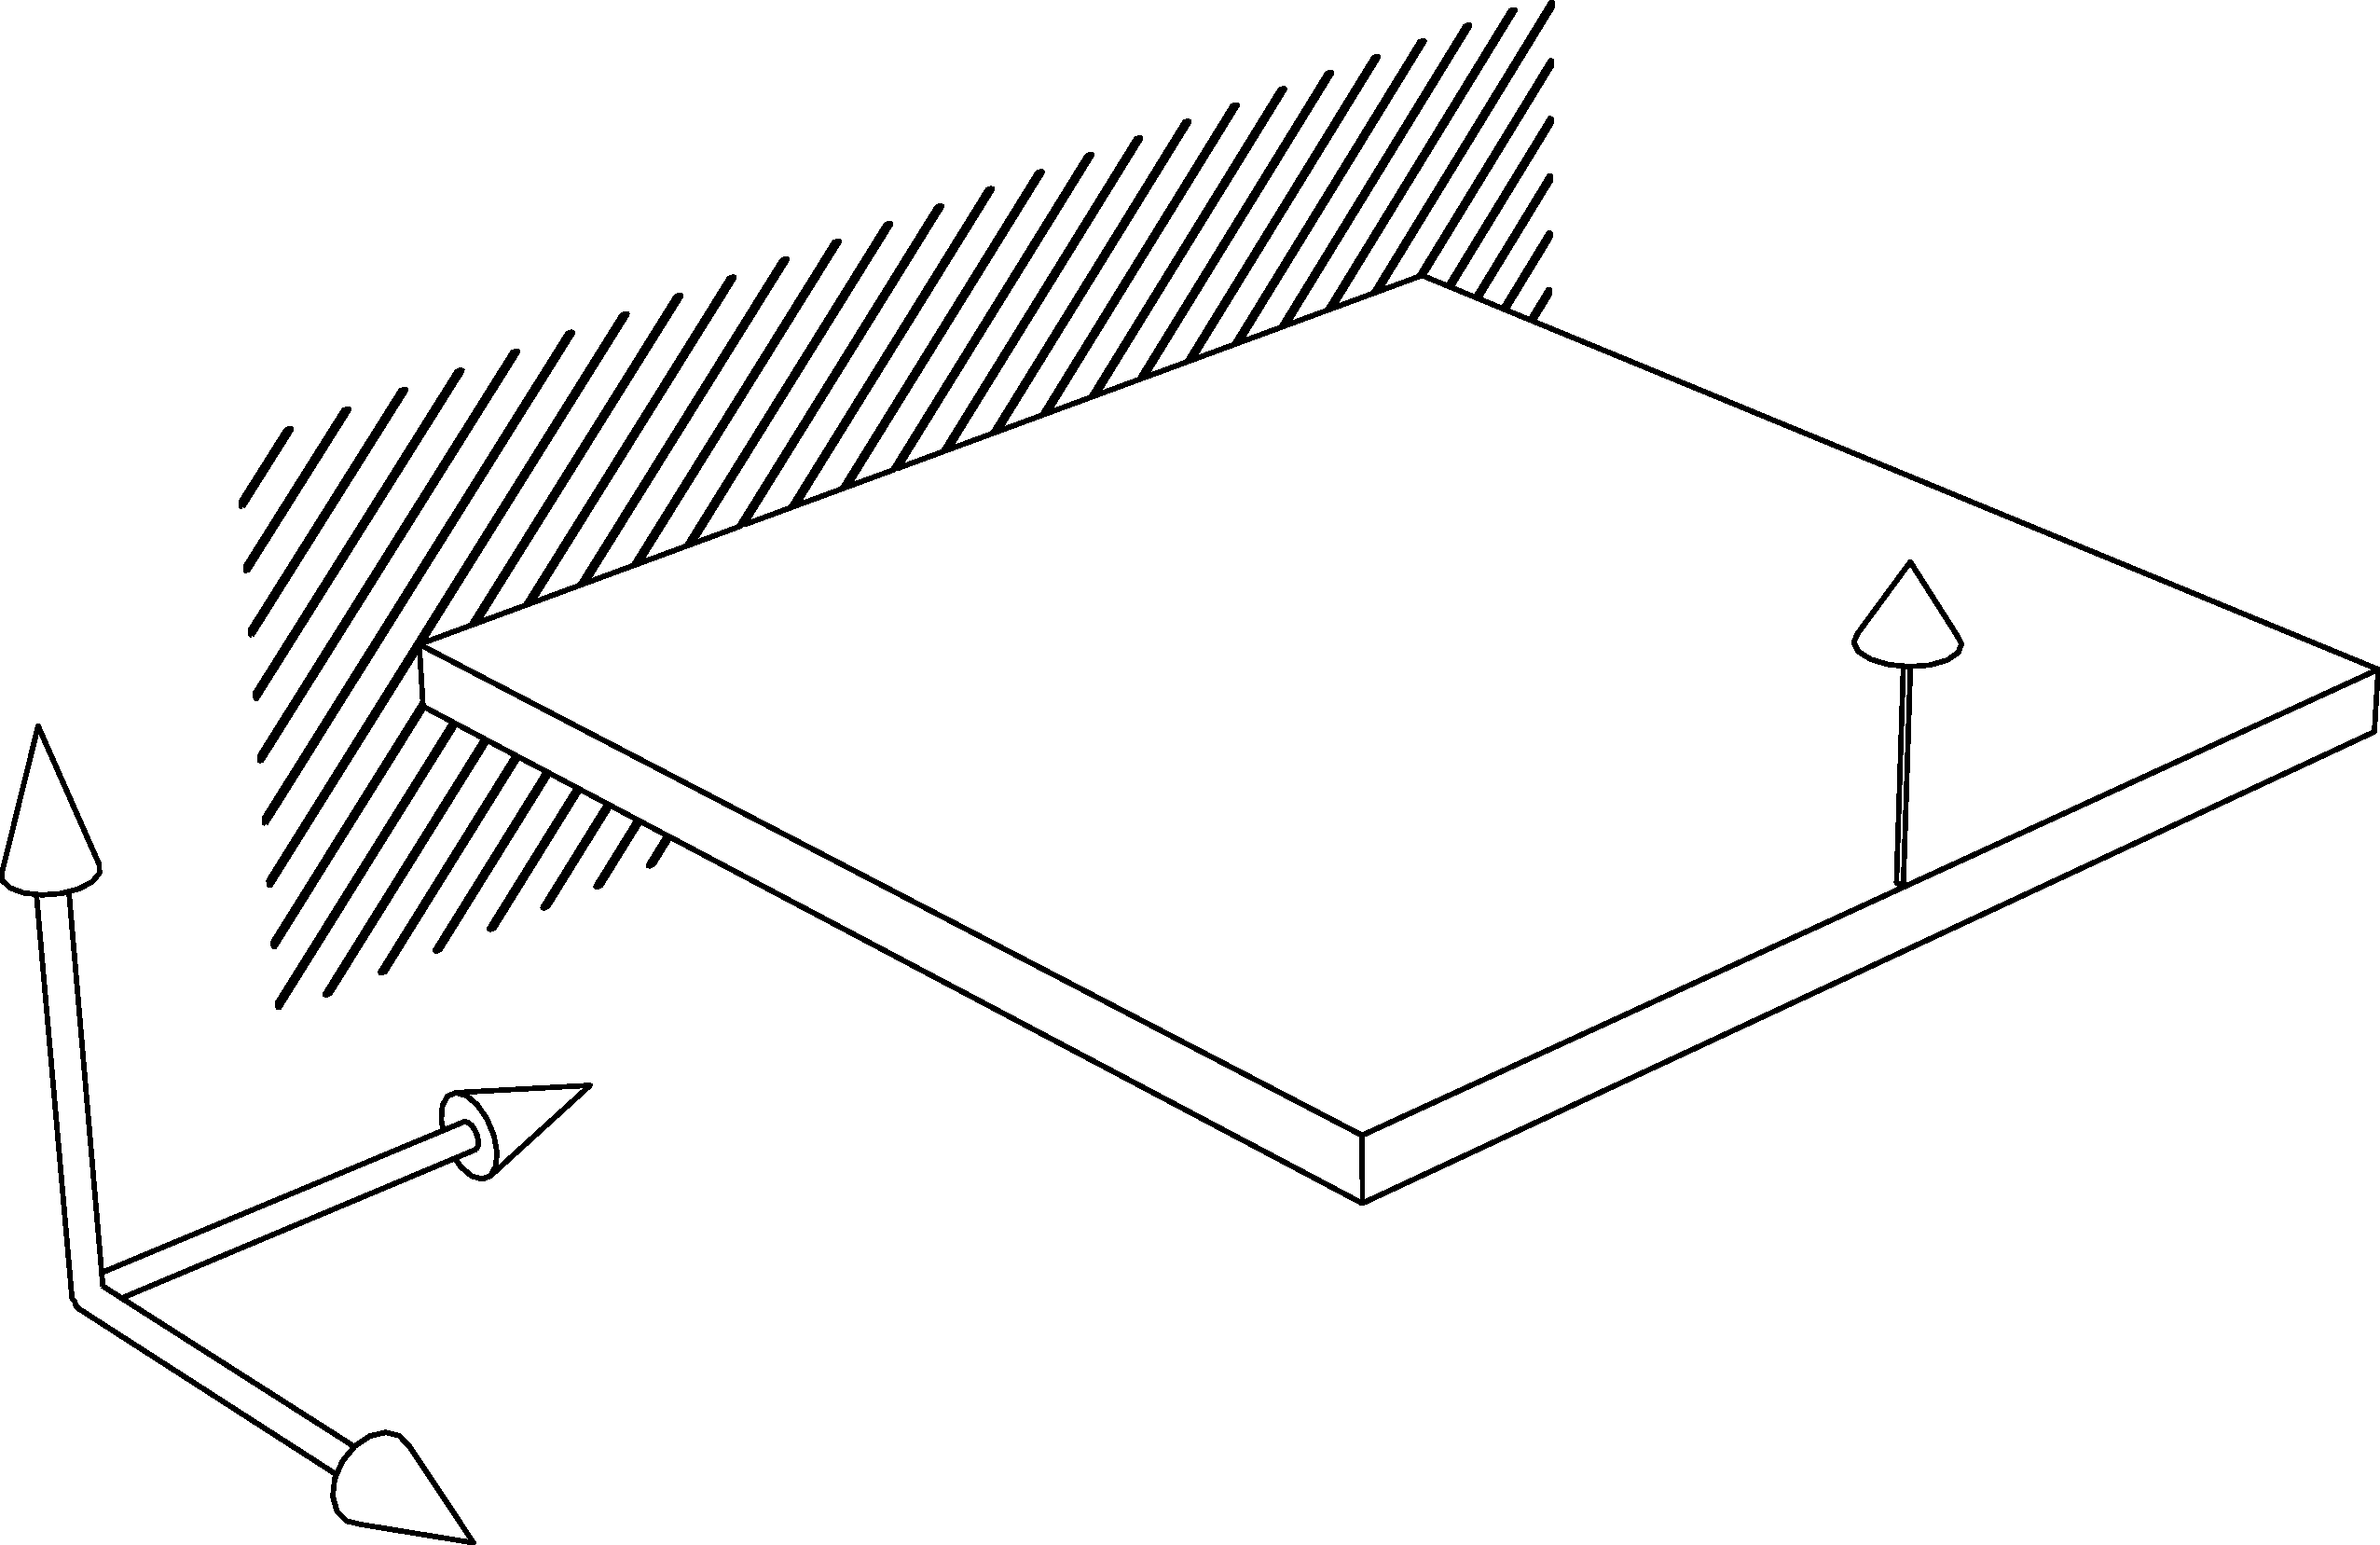
\includegraphics[width=0.4\linewidth]{\currfiledir/bended-plate.blend-min.svg.pdf}};

        \node[] at (-2.8,-2.2) {x};
        \node[] at (-2.0,-1.5) {y};
        \node[] at (-3.7,-0.0) {z};

        \node[rotate=+16] at (-2.4,+1.4) {fixed};

        \node[align=right] at (+0.8,+0.3) {Point A\\$F = \qty{10}{\kilo\newton}$};

        \node[] at (+0.6,-1.4) (A) {};
        \node[] at (+3.5,-0.0) (B) {};
        \node[] at (+1.0,+1.0) (C) {};
        \Dimline[($(A)+(+0.1,-0.1)$)][($(B)+(+0.1,-0.1)$)][below right][\qty{2}{\metre}]
        \Dimline[($(C)+(-0.2,+0.6)$)][($(B)+(+0.1,+0.5)$)][above right][\qty{2}{\metre}]
        \Dimline[($(B)+(+0.5,+0.1)$)][($(B)+(+0.5,+0.3)$)][right][\qty{0.1}{\metre}]

    \end{tikzpicture}
    \caption{Setup of the bended plate test}
    \label{bended-plate:fig:setup}
\end{figure}

\section{Analytical solution}
\label{bended-plate:sec:analytical-solution}

Neglecting geometrical non-linearity, the well-known analytical solution for
the deflection is given in \autoref{bended-plate:analytical-solution}.

\begin{equation}
    \label{bended-plate:analytical-solution}
    u_z = F \cdot \frac{a ^ 3}{3EI} = \qty{0.16}{\metre}
\end{equation}

\begin{samepage}
    with:
    \begin{description}
        \item[$u_{z}$] vertical deflection at the point load to be estimated.
        \item[$F$] point load (\qty{10}{\kilo\newton})
        \item[$a$] size of the plate (\qty{2}{\metre})
        \item[$E$] Young's modulus (\qty[per-mode = symbol]{1E6}{\kilo\newton\per\square\metre}; see \autoref{bended-plate:material-parameters})
        \item[$I$] Second moment of area, for this geometry $I = \frac{b \cdot t^3}{12} = \frac{\qty{2}{\metre} \cdot (\qty{0.1}{\metre})^3}{12} = 0.0001\overline{6} \qty{}{\metre}^4 $
    \end{description}
\end{samepage}

\section{Numerical solution with Moose}
\label{bended-plate:sec:moose}

The discretization of the Moose models are identical to the Plaxis models in
\autoref{bended-plate:sec:plaxis3D}. In fact, the MSH files used by the Moose
models have been created by exporting the Plaxis discretization. Therefore,
several modelling tricks necessary for Plaxis described in
\autoref{bended-plate:sec:plaxis3D} are also imported to Moose even if not
absolutely necessary (e.g. the extension of the shell elements: Moose supports
boundary conditions for the rotation variables).

Currently (begin of 2025), Moose does not offer TRI6 shell elements. To model
this test setup the "Shell MooseApp Code Plugin" to be found in the link below
was used.

\href{https://github.com/Kavan-Khaledi/moose-codeplugin-shell}{github.com/Kavan-Khaledi/moose-codeplugin-shell}

For this purely linear-elastic problem, the ‘NEWTON’ solver is used. The Moose
input files for this model and the corresponding MSH files are attached to this
document as a ZIP by the name of ‘bended-plate.i.zip’. Only one input file is
given for TRI and one for TET elements despite the fact that several
discretizations have been used and all MSH files are given. To reduce the file
size of this document, the reader is requested to adjust the argument pointing
to the MSH file \codeword{[Mesh]/[File]/file} to the desired MSH file.

\fileattachment{\currfiledir/bended-plate.i.zip}{bended-plate.i.zip}

\section{Numerical solution with Plaxis 3D}
\label{bended-plate:sec:plaxis3D}

In order to correctly reproduce the test setup, various tricks had to be used
in the Plaxis models. These tricks include:

\begin{description}
    \item [Shell-Elements:]{To model the fixed end of the plate, Plaxis does not
          support prescribing zero rotation at a ‘Prescribed Line
          Displacement’ boundary condition. Due to this shortcoming
          an ‘extension’ of the plate on the fixed end has been
          modelled and displacement of all nodes of this extension is
          prescribed as zero.\\
          On the other hand, Plaxis suppresses the rotation of all nodes
          of shell elements that are adjacent to the model boundaries (but
          not the displacements). In order to be able to correctly model the
          bending of the plate due to the load, an enveloping volume was
          modeled around the plate, but never activated in the calculation.
          With this trick, none of the nodes of the shell elements touch the
          model boundaries, which means that no unwanted boundary conditions
          are generated.}
    \item [Volume-Elements:]{Plaxis also automatically generates displacement
          boundary conditions for solid elements that touch the model boundaries,
          which are not useful for this model. In the Plaxis models, the
          automatically generated boundary conditions are therefore deactivated,
          displacement boundary conditions are generated manually for the
          boundary surfaces and set to a suitable behavior.}
\end{description}

The Plaxis command files for this model are attached to this document as a ZIP
by the name of ‘bended-plate.p3dlog.zip’.

\fileattachment{\currfiledir/bended-plate.p3dlog.zip}{bended-plate.p3dlog.zip}

Only one input file is given for TRI and one for TET elements despite the fact
several discretizations have been used. To generate the discretizations shown
in \autoref{bended-plate:sec:summary}, the command line that generates the
discretization with the \codeword{_meshd} command must be changed. Only the
first argument of the \codeword{_meshd} command changes and can be taken from
\autoref{bended-plate:tab:plaxis-meshd}.

\begin{table}[htbp]
    \centering
    \caption{Discretization of the ‘bended plate’-models}
    \label{bended-plate:tab:plaxis-meshd}
    \begin{tabularx}{\textwidth}{
            >{\hsize=0.085\hsize\linewidth=\hsize}X
            >{\hsize=0.090\hsize\linewidth=\hsize}R
            >{\hsize=0.080\hsize\linewidth=\hsize}R
            >{\hsize=0.240\hsize\linewidth=\hsize}R
            >{\hsize=0.393\hsize\linewidth=\hsize}Y}

        \hline

        %& CPU-count / wall time (\si{\second}) & RAM (MB)                                                                                             

        Element                         & Element                                             & Node           & DOF                                        & Mesh-Command \\

        Type                            & Count                                               & Count          &                                            &              \\

        \hline

        TRI6                            & \qty{8}{}                                           & \qty{ 48}{}    & $ \textcolor{gray}{\qty{ 48}{} \times 6 =
        }\,\qty{ 288}{} $               & {\texttt{\textcolor{blue}{\_meshd 1.00 256 True 1.2
        0.005}}}                                                                                                                                                           \\

        TRI6                            & \qty{44}{}                                          & \qty{ 464}{}   & $ \textcolor{gray}{\qty{ 464}{} \times 6 =
        }\,\qty{ 2784}{} $              & {\texttt{\textcolor{blue}{\_meshd 0.50 256 True 1.2
        0.005}}}                                                                                                                                                           \\

        TRI6                            & \qty{254}{}                                         & \qty{ 2364}{}  & $ \textcolor{gray}{\qty{ 2364}{} \times 6
        = }\,\qty{ 14184}{} $           & {\texttt{\textcolor{blue}{\_meshd 0.20 256 True 1.2
        0.005}}}                                                                                                                                                           \\

        TRI6                            & \qty{3790}{}                                        & \qty{ 34850}{} & $ \textcolor{gray}{\qty{ 34850}{} \times
        6 = }\,\qty{ 209100}{} $        & {\texttt{\textcolor{blue}{\_meshd 0.05 256 True 1.2
        0.005}}}                                                                                                                                                           \\

        TRI6                            & \qty{23446}{}                                       & \qty{233452}{} & $ \textcolor{gray}{\qty{233452}{}
        \times 6 = }\,\qty{1400712}{} $ & {\texttt{\textcolor{blue}{\_meshd 0.02 256
        True 1.2 0.005}}}                                                                                                                                                  \\

        \hline

        TET10                           & \qty{462}{}                                         & \qty{ 1013}{}  & $ \textcolor{gray}{\qty{ 1013}{} \times 3
        = }\,\qty{ 3039}{} $            & {\texttt{\textcolor{blue}{\_meshd 0.20 256 True 1.2
        0.005}}}                                                                                                                                                           \\

        TET10                           & \qty{3516}{}                                        & \qty{ 3516}{}  & $ \textcolor{gray}{\qty{ 3516}{} \times
        3 = }\,\qty{ 10548}{} $         & {\texttt{\textcolor{blue}{\_meshd 0.05 256 True 1.2
        0.005}}}                                                                                                                                                           \\

        TET10                           & \qty{107819}{}                                      & \qty{158749}{} & $ \textcolor{gray}{\qty{158749}{}
        \times 3 = }\,\qty{476247}{} $  & {\texttt{\textcolor{blue}{\_meshd 0.02 256
        True 1.2 0.005}}}                                                                                                                                                  \\

        \hline
    \end{tabularx}
\end{table}

\section{Summary}
\label{bended-plate:sec:summary}

The Moose and Plaxis models of this appendix use identical discretizations and
can therefore compared directly. In fact, the MSH files have been created by
exporting the Plaxis discretization. \autoref{bended-plate:tab:results} shows
element count, node count, and the deflection of point ‘A’ for the models using
shell elements (TRI6) and volume elements (TET10) for different degrees of
discretization refinement. Visualization of the discretization, initial and
deformed state of the plates can be seen in
\autoref{bended-plate:fig:discretization}.

Main observations are:

\begin{enumerate}
    \item The deflection of point ‘A’ agrees well with the analytical solution for all
          models (TRI6 and TET10).
    \item Compared to the analytical solution, the models with shell elements (TRI6)
          overestimate the deflection in both Moose and Plaxis, except for the coarsest
          model in Moose. However, the shell elements in Moose show a noticeably smaller
          deviation as the analytical solution.
    \item The deflection increases for shell elements (TRI6) with finer discretization in
          Moose, the Plaxis models show no clear trend. When using shell elements, the
          discretization should therefore not be too fine. Even the coarsest Moose model
          shows an acceptable deviation from the analytical solution. However, this
          coincides with the desire to have models with low DOF values in order to limit
          computing times.
    \item The system responses of the models with TET10 elements in Moose and Plaxis are
          de-facto identical.
    \item The deflection determined with TET10 elements provides slightly lower values
          than the analytical solution, whereby the deviation decreases with finer
          discretization.
    \item The good to very good agreement between the numerical solution with TET10
          elements and the analytical solution even for the coarsest discretization
          investigated is taken as an indication that the TET10 elements are less
          susceptible to locking effects. The use of these TET10 elements for
          geotechnical models, even with coarser discretization, should therefore work
          well.
\end{enumerate}

The following statements can be derived from these observations:
\begin{itemize}
    \item If plate-like components are to be modeled with TET10 elements, one element
          layer will be sufficient in most cases.
    \item In view of the results and the fact that the DOF is significantly lower when
          using shell elements, the use of the investigated shell elements (TRI6) for
          plate-like structural components in geotechnical models is recommended.
\end{itemize}

\begin{figure}[htbp]
    \centering
    \begin{tikzpicture}

        \node[inner sep=0pt] (tri6) at (-4.5,0) {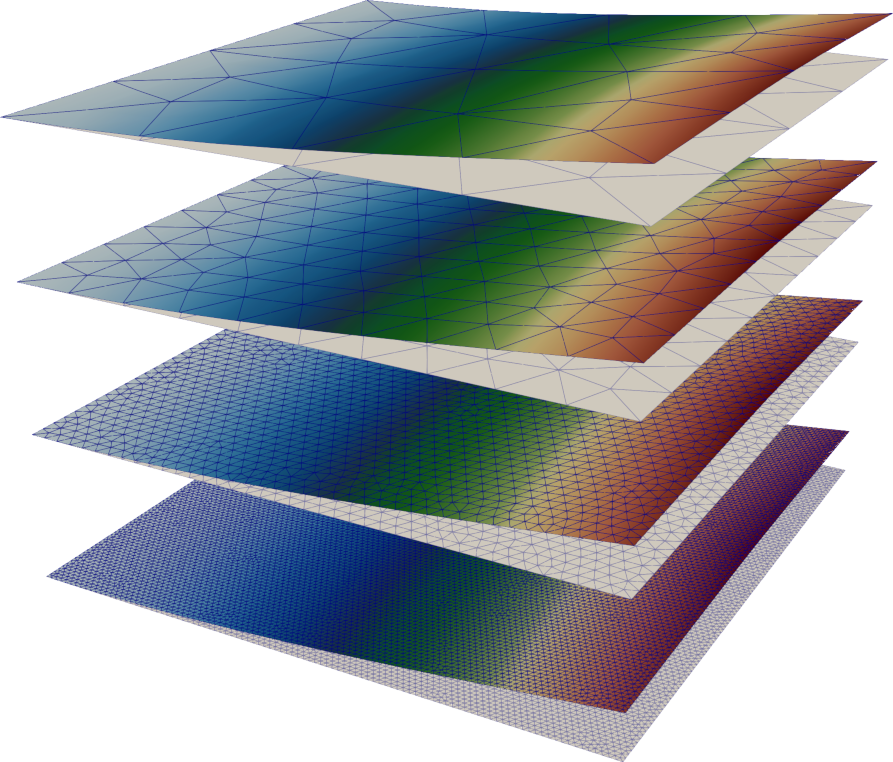
\includegraphics[width=0.45\linewidth]{\currfiledir/bended-plate-tri6-comp.png}};

        \node[inner sep=0pt] (tet10) at (+4.5,0) {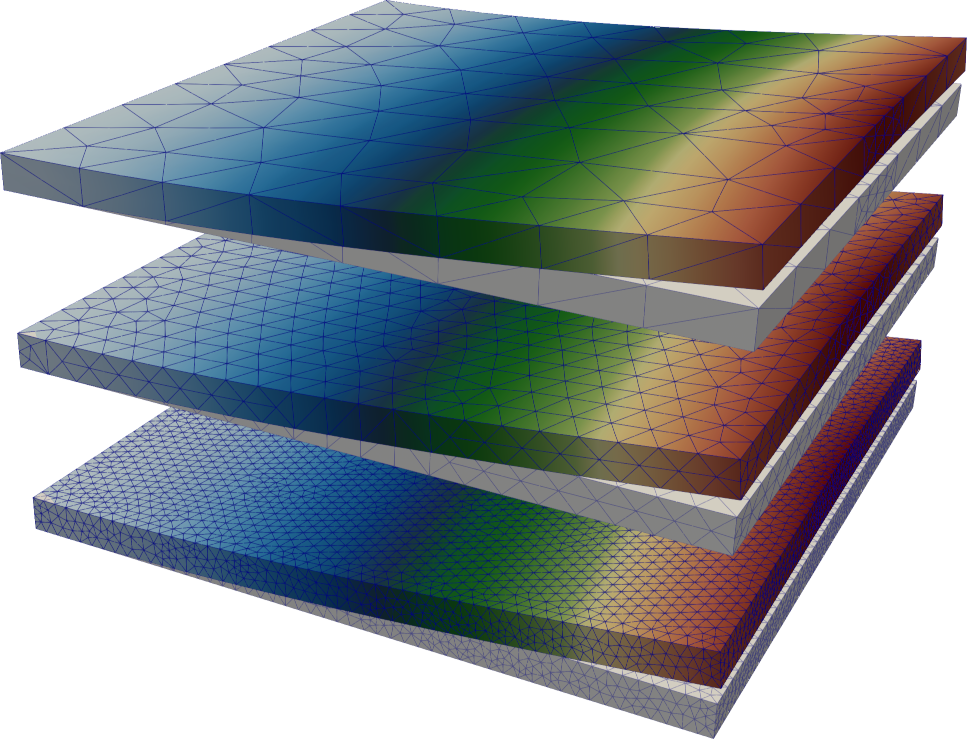
\includegraphics[width=0.45\linewidth]{\currfiledir/bended-plate-tet10-comp.png}};

        \node[rotate=+20] at (-8.0,+3.3) {\tiny\qty{     8}{} TRI6};
        \node[rotate=+22] at (-7.9,+1.9) {\tiny\qty{    44}{} TRI6};
        \node[rotate=+25] at (-7.8,+0.6) {\tiny\qty{   254}{} TRI6};
        \node[rotate=+30] at (-7.7,-0.7) {\tiny\qty{  3790}{} TRI6};
        \node[rotate=+34] at (-7.7,-2.0) {\tiny\qty{ 23446}{} TRI6};

        \node[rotate=+23] at (+1.1,+2.2) {\tiny\qty{   462}{} TET10};
        \node[rotate=+27] at (+1.2,+0.8) {\tiny\qty{  3516}{} TET10};
        \node[rotate=+35] at (+0.9,-0.8) {\tiny\qty{107819}{} TET10};

    \end{tikzpicture}
    \caption{Discretization of the bended plate models (grey: initial; colored: deformed state)}
    \label{bended-plate:fig:discretization}
\end{figure}

\begin{table}[htbp]
    \centering
    \caption{Resulting deflection for selected discretizations (geometrical non-linearity neglected)}
    \label{bended-plate:tab:results}
    \begin{tabularx}{\textwidth}{
            >{\hsize=0.2\hsize\linewidth=\hsize}X
            >{\hsize=0.2\hsize\linewidth=\hsize}R
            >{\hsize=0.2\hsize\linewidth=\hsize}R
            >{\hsize=0.2\hsize\linewidth=\hsize}Y
            >{\hsize=0.2\hsize\linewidth=\hsize}Y}

        \hline

        %& CPU-count / wall time (\si{\second}) & RAM (MB)                                                                                             

        Element & Element        & Node           & \multicolumn{2}{c}{Deflection of Point ‘A’
        (\si{\metre})}                                                                                                \\

        Type    & Count          & Count          & Moose                                      & Plaxis               \\

        \hline

        TRI6    & \qty{8}{}      & \qty{48}{}     & \qty{0.1539}{\metre}                       & \qty{0.1742}{\metre} \\

        TRI6    & \qty{44}{}     & \qty{464}{}    & \qty{0.1646}{\metre}                       & \qty{0.1719}{\metre}
        \\

        TRI6    & \qty{254}{}    & \qty{2364}{}   & \qty{0.1696}{\metre}                       & \qty{0.1712}{\metre}
        \\ % \qty{63}{\mega\byte}

        TRI6    & \qty{3790}{}   & \qty{34850}{}  & \qty{0.1703}{\metre}                       &
        \qty{0.1715}{\metre}                                                                                          \\ % \qty{276}{\mega\byte}

        TRI6    & \qty{23446}{}  & \qty{233452}{} & \qty{0.1704}{\metre}                       &
        \qty{0.1716}{\metre}                                                                                          \\ % \qty{1480}{\mega\byte}

        \hline

        TET10   & \qty{462}{}    & \qty{1013}{}   & \qty{0.1565}{\metre}                       &
        \qty{0.1565}{\metre}                                                                                          \\

        TET10   & \qty{3516}{}   & \qty{3516}{}   & \qty{0.1587}{\metre}                       &
        \qty{0.1587}{\metre}                                                                                          \\

        TET10   & \qty{107819}{} & \qty{158749}{} & \qty{0.1599}{\metre}                       &
        \qty{0.1599}{\metre}                                                                                          \\

        \hline
    \end{tabularx}
\end{table}

\chapter{Bi-axial Shear Test}
\label{app:bi-axial-shear}
\section{Problem statement}

A bi-axial shear test of a homogenous material block of $\SI{1}{\metre} \times
    \SI{1}{\metre} \times \SI{1}{\metre}$ should be modeled to test the limit load
resulting from the Mohr-Coulomb failure criterion. The test setup is shown in
\autoref{bi-axial-shear-mohr-coulomb::fig:setup}. At xmin, ymin, ymax, and zmin
the block is fixed perpendicular to the face. The face xmax is loaded with a
constant (normal) pressure of $\sigma'_2 =
    \qty{1}{\kilo\newton\per\square\metre}$. The (normal) pressure $\sigma'_1$ at
zmax ramps up till no convergence can be found anymore. Material parameters are
givin in \autoref{bi-axial-shear-mohr-coulomb:material-parameters}.

\begin{table}[htbp]
    \centering
    \caption{Material parameters}
    \label{bi-axial-shear-mohr-coulomb:material-parameters}
    \begin{tabularx}{\textwidth}{XYY}

        \hline

        Property                        & Physical unit                                         & Value       \\

        \hline

        Youngs modulus $E$              & \si[per-mode = symbol]{\kilo\newton\per\square\metre} &
        \SI{1000}{}                                                                                           \\

        Poisson's ratio $\nu$           & -                                                     & \SI{0.25}{} \\

        Angle of inner friction $\phi'$ & \si[per-mode = symbol]{\degree}                       & \SI{30}{}
        \\

        Cohesion $c'$                   & \si[per-mode = symbol]{\kilo\newton\per\square\metre} & 1           \\

        \hline
    \end{tabularx}
\end{table}

\begin{figure}[htbp]
    \centering
    \begin{tikzpicture}

        % this image has been generated using Blender writing a SVG
        % using the "Freestyle SVG Exporter". The SVG is minimized
        % using third-party tools and finally converted to PDF using
        % Inkscape.
        \node[inner sep=0pt] (ch-stresses) at (0,0) {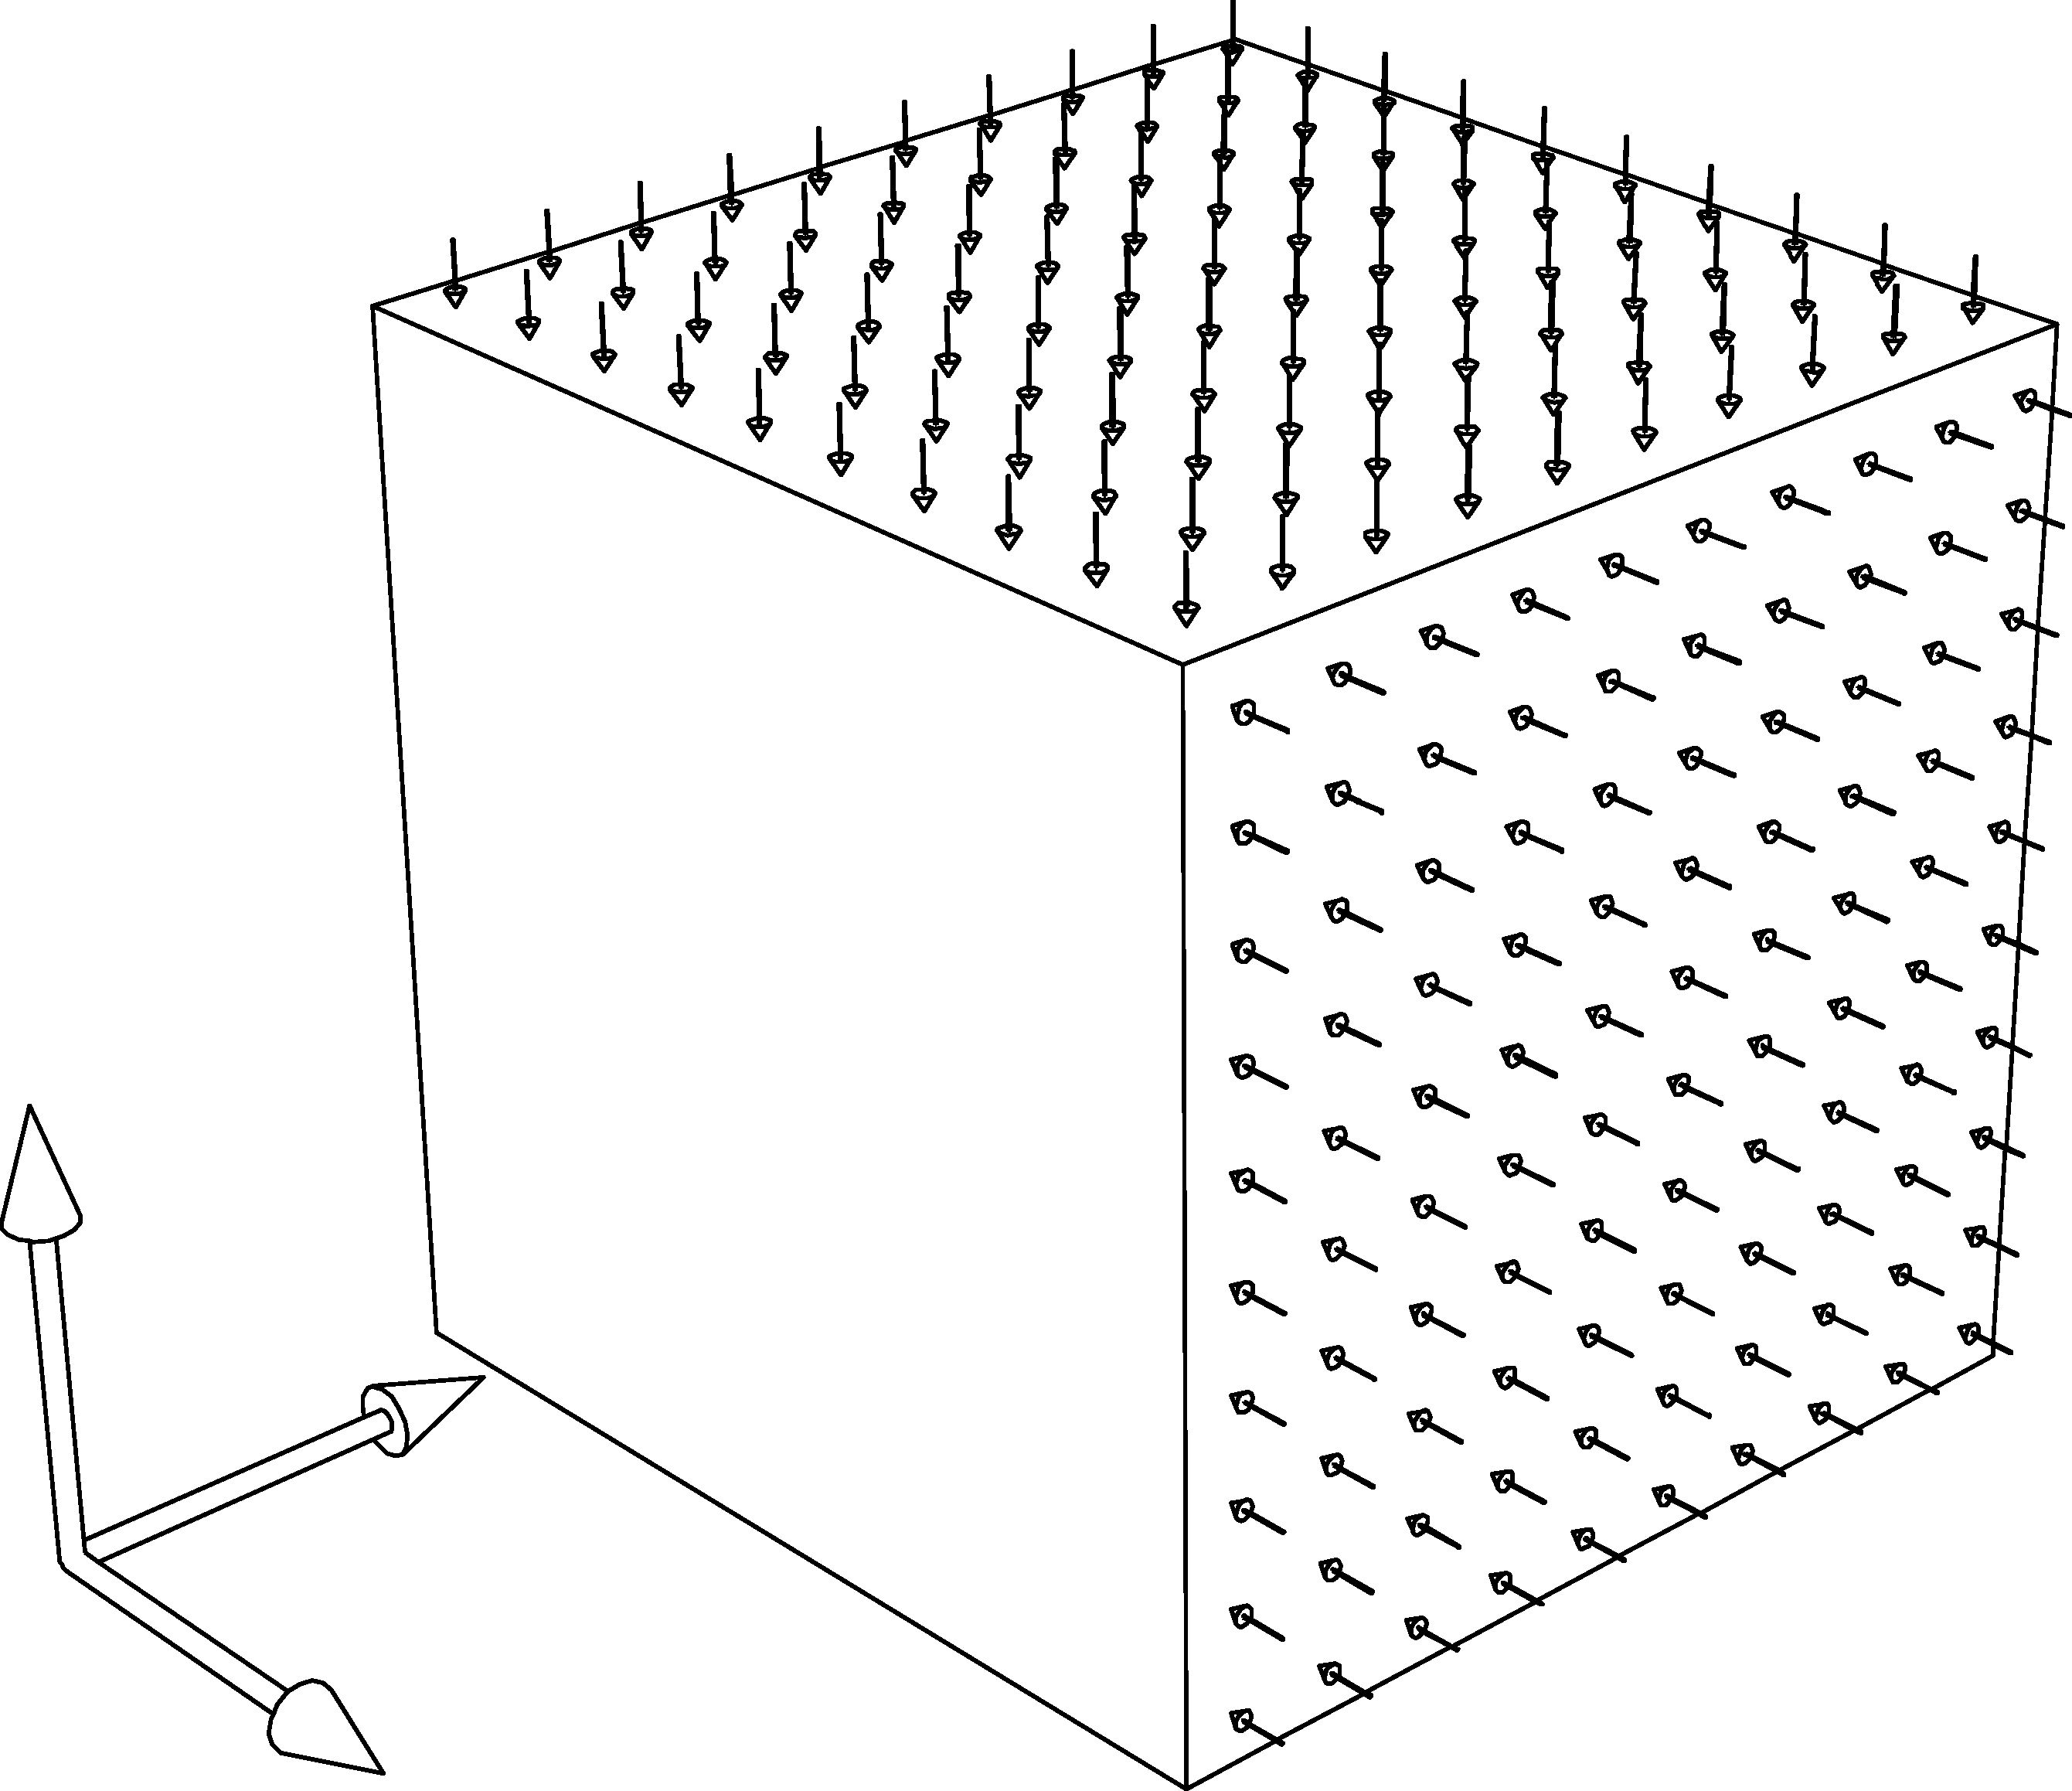
\includegraphics[width=0.4\linewidth]{\currfiledir/bi-axial-shear.blend.svg.pdf}};

        \node[] at (-3.0,-2.9) {x};
        \node[] at (-2.5,-1.5) {y};
        \node[] at (-3.0,-1.0) {z};

        \node[draw,circle,fill=white,minimum size=.5cm,inner sep=0pt, text width=1.5cm, align=center] (xmin_text) at (-4.0,+2.7) {xmin: $u_x \equiv 0$};
        \node (xmin) at (-2.1,+1.2) {};
        \path[->] (xmin_text) edge [out=0, in=180] (xmin);

        \node[draw,circle,fill=white,minimum size=.5cm,inner sep=0pt, text width=2.0cm, align=center] (xmax_text) at (+4.5,-2.5) {xmax: \\ $\sigma'_2 \equiv \qty[per-mode = fraction]{1}{\kilo\newton\per\square\metre} $};
        \node (xmax) at (+2.2,-1.4) {};
        \path[->] (xmax_text) edge [out=180, in=0] (xmax);

        \node[draw,circle,fill=white,minimum size=.5cm,inner sep=0pt, text width=1.5cm, align=center] (ymin_text) at (-3.8,+0.5) {ymin: $u_y \equiv 0$};
        \node (ymin) at (-0.8,-0.7) {};
        \path[->] (ymin_text) edge [out=0, in=180] (ymin);

        \node[draw,circle,fill=white,minimum size=.5cm,inner sep=0pt, text width=1.5cm, align=center] (ymax_text) at (+4.8,+1.7) {ymax: $u_y \equiv 0$};
        \node (ymax) at (+3.3,+0.0) {};
        \path[->] (ymax_text) edge [out=270, in=20] (ymax);

        \node[draw,circle,fill=white,minimum size=.5cm,inner sep=0pt, text width=1.5cm, align=center] (zmin_text) at (-1.2,-3.5) {zmin: $u_z \equiv 0$};
        \node (zmin) at (+0.2,-2.8) {};
        \path[->] (zmin_text) edge [out=0, in=270] (zmin);

        \node[draw,circle,fill=white,minimum size=.5cm,inner sep=0pt, text width=1.2cm, align=center] (zmax_text) at (+2.4,+3.2) {zmax: $\sigma'_1 = ?$};
        \node (zmax) at (+0.4,+1.7) {};
        \path[->] (zmax_text) edge [out=180, in=90] (zmax);

    \end{tikzpicture}
    \caption{Setup of the bi-axial shear test}
    \label{bi-axial-shear-mohr-coulomb::fig:setup}
\end{figure}

\section{Analytical solution}

From the yield function of the Mohr-Coulomb failure criterion shown in
\autoref{eqn:Mohr-Coulomb-failure-criterion} the limit load of the bi-axial
test can be derived as given in \autoref{eqn:bi-axial-test-limit-load}.

\begin{equation}
    \label{eqn:Mohr-Coulomb-failure-criterion}
    f = \frac{\abs{\sigma'_1 - \sigma'_2}}{2} + \frac{\sigma'_1 + \sigma'_2}{2} \cdot \sin{\phi'} - c' \cdot \cos{\phi'} = 0
\end{equation}

\begin{equation}
    \label{eqn:bi-axial-test-limit-load}
    \sigma'_1 = \sigma'_2 \cdot \frac{1 + \sin{\phi'}}{1 - \sin{\phi'}} - 2c' \cdot \frac{\cos{\phi'}}{1 - \sin{\phi'}}
    \approx \qty{-6.464}{\kilo\newton\per\square\metre}
\end{equation}

\section{Moose}

In the corresponding Moose model of this quasi-static problem a discretisation
of \qty{5184}{} TET10 elements and a transient executioner is used. The
linear-elastic material behaviour is modelled with a materials block of type of
\codeword{ComputeIsotropicElasticityTensor}. The ideal-plastic behaviour is
introduced with a materials block of type
\codeword{CappedMohrCoulombStressUpdate}. To avoid the cap of this materials
block to influence the system response, a very high tensile and compressive
strength is used.

The load $\sigma'_1$ ramps up linearly with time so that at $t =
    \qty{6.464}{\second}$ the load is $\sigma'_1 =
    \qty{-6.464}{\kilo\newton\per\square\metre}$. Due to the ideal-plastic nature
of the material behaviour, Moose will attempt to calculate time steps and
iteratively reduce the time step if convergence is not achieved. Eventually the
last converged time step should be at $t \approx \qty{6.464}{\second}$.

This model was calculated using the ‘PJFNK’ solver. The time step is initially
chosen to be \qty{0.25}{\second} and the minimum time step is limited to
\qty{0.001}{\second}. Due to the automatic cut-back of the time steps close to
failure, the last converged time step is at $t=\qty{6.43945}{\second}$. The
Moose input file for this model is attached to this document by the name of
‘bi-axial-shear.i’.

\fileattachment{\currfiledir/bi-axial-shear.i}{bi-axial-shear.i}

\section{Plaxis 3D}

The mesh used for Plaxis3D consists of 5130 TET10 elements.

\end{document}